\chapter{7. Data Analysis and Machine Learning}

In the last two chapters we outlined the portable hardware that was built to measure air quality and push it up to ChainAPI.  We discussed our new backend infrastructure to support air quality data, as well as the tools that were created to allow automatic and extensible machine learning algorithms.  The final element of the system-- and the key element of this project-- is the evaluation of predictive machine learning algorithms in the air quality space.
 
For this test, we were able to co-locate six types of cheap air quality sensor next to EPA reference-level equipment for two months.  In most cases we collected minute-resolution data.  The testing occurred over the course of spring (with high variation in weather as we transitioned from the end of the cold/snowy season to the summer).   

This experimental design gives us the ability to take the difference between our cheap sensor signals and the EPA reference to generate an error signal.  Based on measurements from other sensors on the device in concert with data from external weather APIs, we can apply supervised learning techniques that attempt to predict the magnitude of the error for every reading.  

While there are many potential algorithms we could apply to this problem, for this experiment we simplified our error readings to a binary feature-- indicating whether the cheap sensor was in error or not, based on an appropriate tolerance around the ground truth value.  A logistic regression model-- commonly used for engineering failure prediction-- was selected to predict whether the sensor was in error, as well as assign a probability to this prediction.

<Summary of interesting take aways and results.>

\section{Test Conditions and Data Collection Summary}
 The learnAir V1 sensor was first installed on April 6th, 2016 and taken down on April 14th.  This preliminary test resulted in serious sensor corrosion and unuseable data.

The useful section of the co-location test ran from April 15th to June 13th (59 days).  During that time, several tests were performed.  In total we validated 8 different sensors representing 6 distinct sensor types over periods ranging from 21 to 59 days.  Our co-located test sets range from 1,431 samples of hourly data up to 85,739 samples of minute-resolved data.  


\begin{figure}[htb]
 	\includegraphics[width=\textwidth-0.5cm]{figs/weather}               
 	 \caption{Weather during Test Period.}
  	\label{fig:weather}
\end{figure}


From April 15th through May 23rd (38 days with one 40 minute service break), an older set of AlphaSense O3 and CO electrochemical gas sensors were characterized.  This set was calibrated in Dec 2013 (2 years, 4 months old calibration at the start of the test).  55,589 samples of minute-resolution data was collected to characterize these sensors.

From May 23rd to June 13th (21 days), a brand new set of AlphaSense O3+NO2, NO2, and CO electrochemical gas sensors were characterized (5 month old calibration at the start of the test).  30,150 samples were collected to characterize these sensors.

The two tests of an older and newer set of the same type of Alphasense sensors (O3 and CO) can provide interesting insights-- by comparing the data between the two tests we may be able to draw insights into age- and use-related differences.  By combining the two sets after calibration, we have a long set of data spanning several months to test predictive techniques with.  Assuming the underlying failure modes are the same for sensors of the same make/model, this combined set should be useful at providing insight into the underlying device mechanics.

From April 15th through June 6th (52 days, with two 40 minute service outages), a new SmartCitizen sensor-- with its NO2 and CO sensors-- was installed and running at the MassDEP site.  This sensor gave 85,739 minute-resolved samples.

Finally, from April 15th through June 13th (59 days), our Sharp Particulate Sensor collected samples that we resolved to 1 hour intervals, to match the MassDEP BAM reference.  1,431 samples were collected from this technique.  

\FloatBarrier
\begin{figure}[htb]
 	\includegraphics[width=\textwidth]{figs/weather_summary}               
 	\caption{Temperature and Humidity during Test Period.}
  	\label{fig:weather_summary}
\end{figure}
\FloatBarrier

The co-location tests started with snow on the ground and ended with summer heat.  External temperatures varied from below 5 to above 30 degrees Celcius, and the relative humidity ranged from 20-100\%.  The weather during the period was nicely varied, with a few foggy days, a few windy days, and a particularly rainy week in early May.  See Figures \ref{fig:weather} and \ref{fig:weather_summary} for details, and Appendix D for more information about trends in ambient pressure, dew, light level, precipitation amount, and cloud cover over the course of the testing period.   
\FloatBarrier

\section{Overview of Data Pre-Processing and ML Strategy}
All readings taken by the co-located sensor were measured in 30 second intervals, and timestamped using the on-board Real Time Clock before being saved to an SD card.  Since this was all done offline, no corrections for the timestamps could be applied.

In general, we found a 0.15-0.25\% drift in the RTC timestamps.  This results in 60-200 samples of error every three weeks or so.  To appropriately align these drifted, ~30 second values with our minute-resolved reference values, we applied two stages of correction.  To begin, we corrected the timestamps to reflect their actual time (assuming a constant delay between each, and knowing the precise time the measurements started and ended).  We then linearly interpolated between these corrected timestamp values to find on-the-minute values for every minute.

For the hour long samples of BAM data, we had to consolidate our minute data down to hourly values.  To match the process of the BAM sensor (which collects samples for the first 50 minutes of every hour, and measures for the last ten), we wrote a script to average every value in our machine learning arrays over the course of the first 50 minute of every hour, and throw away the last 10.

This is only the first step of pre-processing the data, however.  For our air quality signals, a calibration step is necessary before comparing the data and characterizing the sensor.  For the SmartCitizen CO and NO2 sensors, as well as for the Sharp particle sensor, their output is an uncalibrated mV value.  In the case of the Sharp sensor, the reading is inverted from the actual particle level (as it is a measure of light that makes it through the sensor without scattering).  These sensors were calibrated using a LMSE approach to optimize a simple scale factor or a scale factor and an offset.  The minimization function was run (1) on all of the data, (2) with the outliers (> 1 stdev) removed, (3) on long-term averages of the data, and (3) to only optimize values that were within some tolerance (throwing out sections that appeared to show disagreement and instead favoring a tighter fit on aligned data).  The most realistic, quality fit was chosen from amongst these options as the `calibrated' reference.

For the AlphaSense sensors, calibration was even more complicated.  These sensors come with a calibration sheet giving appropriate values.  The formula for most of their sensors is: {\small \[ppb = \frac{(we - we_{zero}) - (n*ae - ae_{zero})}{sensitivity}\]} where $we$ is the working electrode measurement in mV, $ae$ is the auxiliary electrode measurement in mV, $we_{zero}$ is the working electrode offset value in mV, $ae_{zero}$ is the auxiliary electrode offset value in mV, $n$ is a temperature dependent and sensor chemistry dependent scale factor, and the sensitivity is the mV/ppb gain factor of the instrumentation amplifier on the conditioning board.  For the cross-sensitive O3+NO2 reading, we use the calibrated NO2 values and subtract the resulting mV offset given the calibrated NO2 sensitivty: {\small \[ppb = \frac{(we - we_{zero}) - (n*ae - ae_{zero}) - \frac{no2_{ppb}}{x\_sensitivity\_to\_no2}}{sensitivity}\]} While we tried the provided calibration data-- as well as simple LMSE scaling-- we found the best agreement came from LMSE minimization using a bounded search of $we_{zero},  ae_{zero},$ and $sensitivity$.  In these cases, the seed values were the provided calibration terms from AlphaSense.  This type of calibration gave very strong results compared to other methods.

With calibrated data, an appropriate tolerance was chosen for each sensor value (typically $\pm$2-5\% of the full range, though a larger tolerance was chosen for particulate), and each reading was classified as `correct' if falling within that tolerance of the MassDEP reference measurement, or `incorrect' if falling outside of it. 

This data is now ready for machine learning using the logistic regression discussed in the introduction to this chapter.  We performed all of this analysis using python's scikit-learn machine learning toolbox-- however, some experimentation was done with the java-based (GUI driven) `Weka' toolkit (using a python ARFF file conversion library), as well as initial exploration with google's new tensor-flow library (which has logistic regression support, but which really shines for its deep learning ability and large dataset handling).  These additions tools, and additional techniques, will be explored in more depth in the near future.

The general outline of the machine learning process we applied to the data is as follows: (1) load in the feature values (approximately 150 of them) to predict our binary error classification, (2) impute (or fill in) missing values, (3) split our data into training and test sets used 5-fold cross-validation, (4) run a grid search over logistic regression parameter-space to find the best regularization coefficient and penalty terms, (5) train our new 'best model' using the five training sets, and (6) verify the results on the five test sets.  Importantly, two types of cross-validation are used-- a shuffled type and a chunked type.  In one case, data from the entire two month period is randomly selected to constitute training and test sets; in the other, the first several weeks are used to predict the last, the last several are used to predict the first, etc.  The difference in these results gives us important insight into algorithm robustness and the effect of seasonal variation on our predictions.  

Additionally, we use randomized decision trees to rank the importance of our features, as well as seven other feature reduction techniques (correlation, linear regression, random forest, lasso, RFE, ridge, and stability).  A reduced set of the top 15 features is then used to retrain our original Logistic Regression, and the results are compared.  The strength of agreement between feature reduction techniques can suggest meaningful predictive relationships, and the relative strength of the classifier with this reduced feature set can also corroborate strong causality for the top features.

There are two main metrics we use to evaluate our system performance.  The most obvious metric is to compare the right answer ('is the sensor actually in error?') with the predicted one ('do we think the sensor is in error?') and display our results in a 2x2 confusion matrix.  We can easily calculate the error rate of our algorithm from this matrix.

Logistic Regression offers a probability along with its prediction, however, so to fully evaluate the strength of our results we must take these probabilities into account.  Our second evaluation metric-- and the accepted standard for this type of evaluation-- is a Receiver Operating Characteristic (ROC) curve.  This curve plots the true positive rate (the number of correct predictions that a measurement is in error, normalized by the total number of errored air quality readings) against the false positive rate (the number of incorrect predictions that a measurement is in error normalized by the total number of accurate air quality readings).  We can compute a point on this graph by choosing an arbitrary threshold for our probability, and classifying every measurement as a predicting an error in our reading or not based on whether the probability that it is falls above or below this threshold value.  If we set our probability threshold at 50\%, we find the point corresponding to our original confusion matrix.

When we plot the points for every threshold value (from 0-100\%), we generate an ROC curve.  These curves start at (0,0) and end at (1,1) on our plot.  Random guessing will form a line between the points at a 45 degree angle.  Perfect accuracy with 100\% confidence will form a right triangle-- jumping immediately to a value of (0,1) on our graph before continuing horizontally over and meeting up with the upper right corner.  Real, meaningful predictions will likely fall somewhere in between.  The area under the ROC curve (AUC-ROC) is normalized to a value between 0 and 1, and frequently used to characterize the quality of predictions generated by our logistic regression in a more comprehensive way than a simple confusion matrix.  Generally speaking, values above 0.8 suggest our model has good-to-excellent predictive power as the number grows closer to one, and values above 0.7 represent reasonable predictions.  Values below this mark are marginal, with anything close to 0.5 suggesting total failure.

Once we've found the AUC-ROC for our optimized logistic regression, we compare the results for the 5-fold validation sets (one having been `shuffled' or randomized, and the other having been `chunked').  The shuffled version assumes no time dependent phenomena-- using randomly chosen samples throughout the entire test to predict random other samples interspersed throughout the test.  The chunked version is a more realistic model-- using data we've already gathered from one period of time to predict future data.  

We must be careful with the shuffled version-- errors frequently occur together in time (a sensor will misread for an hour or two in a row, giving a few hundred errors at once, likely because of underlying phenomena).  Monotonically increasing functions (like temperature) could serve as a proxy for time, and the algorithm might take advantage of this co-occurance to `predict' our error.  This is a classic example of overfit, and it should be simply to look at the underlying feature and error distributions to ensure that our model hasn't led us to incorrect conclusions.  This could lead to artificially strong results in the shuffled case.  If we see a strong predictive relationship for one of these variables in the shuffled case, it is important to make sure that the variable is not simply monotonic and co-occuring with one large window of consecutive poor readings.  

After verifying the quality of our shuffled results, we can compare the shuffled and blocked versions of the algorithm.  If the shuffled version still does substantially better than the block-wise version, it suggests that we haven't trained on enough data to capture season-agnostic predictive information.  However, when the two agree, it forms a powerful indication that (1) we've captured enough data to train across seasons, and (2) we have hit upon real and useful phenomena.  
\FloatBarrier

\section{Machine Learning Features}
In most of these applications, around 150 features were used to train our machine learning algorithms.  Features were either measured from the learnAir system or harvested from the Forecast.IO weather API.  A few additional features (the EPA reference black carbon, wind speed, and wind direction measurements) were all included as training features.  Raw sensor signals are included as well as their calibrated versions.  Many of these signals were further manipulated or processed to give more derived features.  

The measured set of features represents data collected from on-board sensors-- temperature, humidity, noise, light, vibration, pressure/airflow, and other air pollution sensors.  We also include the signal from the sensor whose quality we're trying to predict as well (if it reads in certain ranges or slews at a certain rate, we may be able to assume that the sensor is out of its useful range).  

For most of the main features, we created derivative features to predict errors resulting from rapid changes in environmental conditions (anecdotally, we know this to be true for electrochemical sensors).  We also looked at intelligently chosen averages over time-- ones that minimized quantization errors, smoothed data to match the EPA reference, or whose averaging gave evidence of longer term trends that might also be important in analyzing sensor state and measurement quality.

\begin{marginfigure}
 	\includegraphics[width=\textwidth]{figs/humidity_derivative}               
 	 \caption{Humidity Derivative Feature Creation}
  	\label{fig:humidity_derivative}
\end{marginfigure}

\begin{figure}[htb]
\centering
 	\includegraphics[width=\textwidth-2cm]{figs/temp_derivative}               
 	 \caption{Temperature Derivative Feature Creation}
  	\label{fig:temp_derivative}
\end{figure}



Several API's were evaluated for use in this project, and Forecast.IO stood out as a well-reputed option.  They use machine learning to combine many weather forecast APIs into one highly accurate dataset.  The Forecast.IO data comes in hourly intervals, so a running 60 minute average was used to interpolate the values to minute resolution (most of the measured fields, like temperature, are relatively slow-moving).  For class-based indicators (for instance, the `weather-summary' field indicating `cloudy', `windy', `foggy', `rainy', etc) we converted the API value into binary fields that matched each class.   

We created features such as `temperature differential' and `humidity differential' -- a constructed feature that corresponds to the difference in measurement between the ambient conditions (as measured by Forecast.IO) and the conditions in the box (as measured by the SmartCitizen Kit).  While these features are linear combinations of other features (and thus won't improve our model's predictive power), they serve an intuitive purpose, and may help reduce the feature set (mapping two features to one) if they turn out to be important indicators of performance.
 
\begin{figure}[htb]
\centering
 	\includegraphics[width=\textwidth-2cm]{figs/temp_daily}               
 	 \caption{Temperature Inside vs. Outside the Device during Test Period}
  	\label{fig:temp_daily}
\end{figure}

\begin{figure}[htb]
\centering
 	\includegraphics[width=\textwidth - 2cm]{figs/humidity_daily}               
 	 \caption{Humidity Inside vs. Outside the Device during Test Period}
  	\label{fig:humidity_daily}
\end{figure}

Finally, we added some features to represent other potentially important quantities.  These features include the time of day (including features for morning and evening rush hours), the day of the year (mapping to the season), and the elapsed time since the device was plugged in (for `warming up' effects).

In general, some small subset of features was removed for each training session.  For instance, the higher quality Alphasense CO sensor was removed as a feature when training the less capable SmartCitizen CO sensor.  (Training with this feature gives incredibly high accuracy at predicting failure, because it is effectively training itself with the answer.)  By training with comparable or cheaper sensors, we can assess the likelihood of a cheap system working predictably.

In most cases, the EPA reference black carbon sensor data was left as a feature-- while this is not a feasible measurement for a portable, cheap device, it is still useful to know if black carbon is a strong predictor of a sensor's failure.  This knowledge allows us to infer something about how the sensor is failing, and what type of sensor we might want to pair it with.  With this technique, the machine learning process is not evaluative of a current system's success-- instead, it works as an exploratory tool that might inform a potential system design.

The next page includes a list of the main features.  Processed, calibrated, and other derived features extend this list to the complete set.  For histogram plots of many of the main features (made using Weka), see Appendix D.

\begin{table}[H]
\small
\centering
\begin{tabular}{lclc|c|}
\\
\\
\toprule
Feature & Type & Description \\
\midrule
AlphaSense \#1 Work Electrode & Continuous & raw signal from alphasense sensor \\
AlphaSense \#1 Aux Electrode & Continuous & raw signal from alphasense sensor \\
AlphaSense \#2 Work Electrode & Continuous & raw signal from alphasense sensor \\
AlphaSense \#2 Aux Electrode & Continuous & raw signal from alphasense sensor \\
AlphaSense \#3 Work Electrode & Continuous & raw signal from alphasense sensor \\
AlphaSense \#3 Aux Electrode & Continuous & raw signal from alphasense sensor \\
AlphaSense O3 & Continuous & calibrated signal from raw electrode readings \\
AlphaSense NO2 & Continuous & calibrated signal from raw electrode readings \\
AlphaSense CO & Continuous & calibrated signal from raw electrode readings \\
AlphaSense H2S & Continuous & calibrated signal from raw electrode readings \\
AlphaSense Temperature & Continuous & raw signal from alphasense temp sensor \\
Wind Pressure Reading & Continuous & raw signal from pressure sensor \\
Corrected Wind Reading & Continuous & conditioned pressure signal to relate to wind \\
Sharp Dust Reading & Continuous & raw signal from optical particulate sensor \\
SmartCitizen CO Voltage & Continuous & raw signal from smartCitizen CO sensor \\
SmartCitizen NO2 Voltage & Continuous & raw signal from smartCitizen NO2 sensor \\
SmartCitizen Noise Voltage & Continuous & raw signal from smartCitizen Piezo mic \\
SmartCitizen Humidity Voltage & Continuous & raw signal from smartCitizen SHT15 \\
SmartCitizen Temperature Voltage & Continuous & raw signal from smartCitizen SHT15 \\
SmartCitizen Humidity & Continuous & conditioned smartCitizen Humidity Measurement \\
SmartCitizen Temperature & Continuous & conditioned smartCitizen Temperature Measurement \\
SmartCitizen Light Reading & Continuous & raw signal from smartCitizen light sensor \\
SmartCitizen Solar Panel Charge & Continuous & raw signal from smartCitizen sensor \\
EPA Sensor Wind Direction & Continuous & calibrated, accurate EPA reference measurement \\
EPA Sensor Wind Speed  & Continuous & calibrated, accurate EPA reference measurement \\
EPA Sensor Black Carbon  & Continuous & calibrated, accurate EPA reference measurement \\
ForecastIO Apparent Temperature & Continuous & calibrated api call measurement \\
ForecastIO Cloud Cover & Continuous & calibrated api call measurement \\
ForecastIO Dew Point & Continuous & calibrated api call measurement \\
ForecastIO Humidity & Continuous & calibrated api call measurement \\
ForecastIO Precipitation Intensity & Continuous & calibrated api call measurement \\
ForecastIO Precipitation Probability & Continuous & calibrated api call measurement \\
ForecastIO Pressure & Continuous & calibrated api call measurement \\
ForecastIO Temperature & Continuous & calibrated api call measurement \\
ForecastIO Visibility & Continuous & calibrated api call measurement \\
ForecastIO Wind Bearing & Continuous & calibrated api call measurement \\
ForecastIO Wind Speed & Continuous & calibrated api call measurement \\
ForecastIO Clear Night & Boolean & calibrated api call measurement \\
ForecastIO Clear Day & Boolean & calibrated api call measurement \\
ForecastIO Partly Cloudy Day & Boolean & calibrated api call measurement \\
ForecastIO Partly Cloudy Night & Boolean & calibrated api call measurement \\
ForecastIO Cloudy & Boolean & calibrated api call measurement \\
ForecastIO Rainy & Boolean & calibrated api call measurement \\
ForecastIO Foggy & Boolean & calibrated api call measurement \\
ForecastIO Windy & Boolean & calibrated api call measurement \\
Morning Hours & Boolean & created field to correspond to the morning \\
Afternoon Hours & Boolean & created field to correspond to the afternoon \\
Evening Hours & Boolean & created field to correspond to the evening \\
Morning Rush Hours & Boolean & created field to correspond to the morning rush \\
Lunch Hours & Boolean & created field to correspond to the lunch \\
Evening Rush Hours & Boolean & created field to correspond to the evening rush \\
Day Hours & Boolean & created field to correspond to the day \\
Night Hours & Boolean & created field to correspond to the night \\
Outside and Inside Box Temp Differential & Continuous & Difference between temp out/in box \\
Minutes Since Plugged In & Continuous & to help quantify initial terrible readings as sensor settles \\
Day of Year & Continuous & day resolution proxy for seasonality \\
\bottomrule
\end{tabular}
\label{tab:feature_table}
\caption{Machine Learning Features used to Predict Sensor Accuracy}
\end{table}



\FloatBarrier

\section{SmartCitizen CO}
One SmartCitizen CO sensor was tested against the EPA reference.  It was 1 month old at the time of installation, and ran for 52 days (from 4/15 - 6/6 2016) with two ~40 minute service interruptions.  This test gave 74,961 samples of minute resolution data for this machine learning task.


\subsection{Pre-processing}

\begin{marginfigure}
 	\includegraphics[width=\textwidth]{figs/co_sck_zoomed}               
 	 \caption{SmartCitizen CO Raw Data (orange) vs. EPA reference (green)}
  	\label{fig:sck_co_raw_zoomed}
\end{marginfigure}

The SmartCitizen CO sensor data comes uncalibrated, as a mV value that should correlate to CO concentration.  The first step was to run a bounded LMSE minimization on the data in order to scale and offset it appropriately to match the real data.  You can see the final result of such a scaling in Figure \ref{fig:sck_co_with_7p5_accuracy_zoomed}.  You'll notice that the LMSE minimization basically scaled the sensor values down to a minimal amount of variation.  This suggests that the sensor data itself is relatively useless in this context, which is relatively unsurprising given its working range and the near constant <1 ppm exposure.  

Interestingly, the SCAQMD (South Coast Air Quality Management District) showed good correlation for 5-minute average, 500-1000 ppb range over their ten day co-location study.  Our measurements were a few hundred ppb lower on average.  It's also unclear which version of the Smart Citizen sensor SCAQMD tested, as Smart Citizen released an updated version of their board with completely different CO and NO2 gas sensors.  It appears likely, given the test date, that they were using a different (though similarly priced) sensor module entirely.


\FloatBarrier
\subsection{Machine Learning}


Machine learning on this data will tell us effectively nothing about the sensor's accuracy, since the sensor's correlation to the correct values is so poor.  We don't need machine learning to see that the sensor has failed to predict meaningful values.  Instead, applying machine learning here reduces to a comparison of the real CO concentration to a (more or less) constant baseline-- this means our machine learning techniques simply attempt to predict when transients and elevated levels of CO occur at this location using metrological and other sensor data. 


\begin{figure}[htb]
 	\includegraphics[width=\textwidth]{figs/sck_co_with_7p5_accuracy_zoomed}               
 	 \caption{SmartCitizen CO with 7.5\% Accuracy Threshold}
  	\label{fig:sck_co_with_7p5_accuracy_zoomed}
\end{figure}

In this case, the threshold for an `accurate' reading made by the SmartCitizen CO sensor was set at 7.5\% (or $\pm$3.75\%) of the full range of values detected for the actual CO levels, ~315 ppb ($\pm$157.5 ppb).   Figure \ref{fig:sck_co_with_7p5_accuracy_zoomed} shows the Smart Citizen values against the reference, with `accurate' measurements highlighted with a green background.  The `inaccurate' readings are the peaks and large diversions from the baseline.

As with all of the machine learning models, scikit learn was used to conduct a parameterized search for the optimal logistic regression was conducted using parameters C = [0.001, 0.1, 10, 1000] and penalty-type=['L1', 'L2'] with a 2-fold cross-validation.  This covers a reasonable amount of parameter space for the minimal 16 rounds of training and validation (~1-2 hours on my i5 laptop).  For this test, an L1 penalty and C=10 regularization term gave the best ROC\_AUC score of 0.82.  


\begin{table}[]
\centering
\begin{tabular}{|c|c|c|c|c|}
\toprule
\multicolumn{5}{|c|}{Error Rates for SmartCitizen CO with Logistic Regression} \\
&\multicolumn{2}{|c|}{all features} & \multicolumn{2}{|c|}{top 15 features} \\
&shuffled & chunked & shuffled & chunked \\
avg & 0.09 & 0.09 & 0.09 & 0.09 \\
min & 0.08 & 0.03 & 0.09 & 0.08 \\
max & 0.09 & 0.12 & 0.09 & 0.11 \\
\bottomrule
\end{tabular}
\label{tab:sck_co_error_rates}
\caption{Error Rates for Predicting SmartCitizen CO Accuracy with Logistic Regression}
\end{table}

We see similar error rates of about 9\% error in our predictions regardless of whether we chunk or shuffle the data, or whether we use the full set of ~150 features or just a subset of the top fifteen.  The average confusion matrix (five shuffled trained sets validated on a new 1/5 of the full data-set each time) is shown in Table \ref{tab:sck_co_confusion}.  The confusion matrix for the chunked set has similar values.

\begin{margintable}[]
\centering
\offinterlineskip
\hspace*{-5cm}\raisebox{-4cm}[0pt][0pt]{\rotatebox[origin=c]{90}{\parbox[c][0pt][c]{3cm}{\textbf{Actual Values}\\[20pt]}}}\par
\hspace{.3cm}\MyHBox[\marginparwidth]{Predicted Values}\par
\vspace{-.5cm}
\hspace*{1cm}\MyHBox{0}\MyHBox{1}\par
\MyTBox{0}{197.0}{1187.4}
\vspace{-.35cm}\MyTBox{1}{108.6}{13499.2}\raisebox{-1cm}
}
\label{tab:sck_co_confusion}
\caption{Average SmartCitizen CO Confusion Matrix w/Shuffled K-Fold}
\end{margintable}

Though these conditions look the same based on average error rate and confusion matrix, when we examine the confidence of our predictions we see some dramatic differences in the shuffled vs. chunked cases.  From Figure \ref{fig:sck_co_7p5_roc} we can see the shuffled tests resulted in strong, consistent AUC-ROC scores between 0.81 and 0.83, while the chunked version resulted in unconvincing, highly variable results from 0.43 (worse than uneducated guessing) to 0.76.  When using only the top 15 features from a random tree algorithm, we see similar trends, however our accuracy drops from slightly above 0.8 to slightly about 0.7 for the shuffled case (see Appendix D for a list of the top features selected in this way, and a graph of ROC results for the same algorithm using just those features).   

\begin{figure}[htb]
 	\includegraphics[width=\textwidth]{figs/sck_co_7p5_roc}               
 	 \caption{SmartCitizen CO ROC Curve}
  	\label{fig:sck_co_7p5_roc}
\end{figure}

\begin{table}[]
\centering
\small
\begin{tabular}{lllllllll}
\\
\\
\toprule
     & Corr. & Lasso & Lin Reg & RF   & RFE  & Ridge & Stability & Mean \\
\midrule
bkcarbon                            & 1     & 0          & 0    & 1    & 0.58  & 0.28      & 0.93 & 0.54 \\
avg\_60\_bkcarbon                   & 0.98  & 0          & 0    & 0.25 & 0.53  & 0.15      & 0.83 & 0.39 \\
evening                             & 0.17  & 0          & 0.07 & 0.19 & 0.82  & 0.18      & 1    & 0.35 \\
avg\_1440\_bkcarbon                 & 0.57  & 0          & 0    & 0.37 & 0.53  & 0.44      & 0.54 & 0.35 \\
humidity\_box\_differential         & 0.1   & 0          & 0.01 & 0.22 & 1     & 1         & 0.02 & 0.34 \\
afternoon                           & 0.17  & 0          & 0.07 & 0    & 0.84  & 0.19      & 1    & 0.32 \\
avg\_60\_forecastio\_humidity       & 0.01  & 0          & 0.01 & 0.12 & 1     & 1         & 0    & 0.31 \\
temp\_sck\_box\_differential        & 0.09  & 0          & 0    & 0.45 & 0.84  & 0         & 0.73 & 0.3  \\
Solar Panel ( V)                    & 0.05  & 0          & 1    & 0    & 0.77  & 0         & 0    & 0.26 \\
avg\_720\_bkcarbon                  & 0.65  & 0          & 0    & 0.26 & 0.27  & 0.14      & 0.43 & 0.25 \\
forecastio\_apparentTemperature     & 0.04  & 1          & 0    & 0.03 & 0.16  & 0         & 0.43 & 0.24 \\
lmse\_avg\_30\_scaled\_arduino\_ws  & 0     & 0          & 0    & 0.05 & 0.8   & 0.03      & 0.79 & 0.24 \\
forecastio\_clear-night             & 0     & 0          & 0.08 & 0.04 & 0.91  & 0.06      & 0.51 & 0.23 \\
forecastio\_partly-cloudy-day       & 0.06  & 0          & 0.08 & 0    & 0.91  & 0         & 0.55 & 0.23 \\
forecastio\_partly-cloudy-night     & 0.01  & 0          & 0.08 & 0    & 0.89  & 0.06      & 0.54 & 0.23 \\
avg\_30\_scaled\_arduino\_ws        & 0     & 0          & 0.02 & 0.07 & 0.81  & 0         & 0.74 & 0.23 \\
Noise ( mV)                         & 0.02  & 0          & 0    & 0.11 & 0.39  & 0.02      & 0.92 & 0.21 \\
avg\_720\_lmse\_scaled\_sharpDust   & 0.03  & 0          & 0    & 0.15 & 0.55  & 0.22      & 0.52 & 0.21 \\
derivative\_avg\_720\_bkcarbon      & 0     & 0          & 0    & 0.12 & 0.63  & 0.25      & 0.45 & 0.21 \\
daily\_avg\_sck\_humidity           & 0.07  & 0          & 0    & 0.18 & 0.59  & 0.17      & 0.4  & 0.2  \\
derivative\_avg\_360\_lmse\_as\_no2 & 0     & 0          & 0    & 0.11 & 0.55  & 0.73      & 0    & 0.2  \\
derivative\_avg\_1440\_bkcarbon     & 0.02  & 0          & 0    & 0.14 & 0.64  & 0.02      & 0.58 & 0.2  \\
evening\_rush                       & 0.13  & 0          & 0    & 0.04 & 0.49  & 0.1       & 0.54 & 0.19 \\
avg\_60\_forecastio\_pressure       & 0.07  & 0          & 0    & 0.26 & 0.41  & 0.01      & 0.6  & 0.19 \\
\bottomrule
\end{tabular}
\label{tab:sck_co_top_features}
\caption{Top Features for Predicting SmartCitizen CO}
\end{table}

Table \ref{tab:sck_co_top_features} shows the top features for predicting CO variations away from the baseline, as determined by seven different feature reduction techniques.   

The top features-- combined with our ROC results-- give us insight into the usefulness of this algorithm for predicting transient fluctuations in CO.  The large divergence between shuffled and chunked data suggests we have not collected enough data yet to make seasonally-agnostic predictions in CO.  However, the promising results in our shuffled data lead us to believe it is possible to make fairly robust predictions (within or accounting for the season) with enough data collection.  The relationships we find in our shuffled results are consistent and reliable across test sets.  

The top features include black carbon readings, time of day designations (like evening or night), windspeed measured at the sensor, and temperature.  These are in line with expectation-- as a similar combustion byproduct, we would expect black carbon and CO to be closely related.  Heavy traffic (the main source of both black carbon and CO) has predictable time-of-day patterns.  Temperature and windspeed have been directly correlated to changes in CO concentration, given a constant, predictable source.   Furthermore, we'd expect our prediction to be based on a complex relationship of many underlying features.  The difference in results from the full feature set to the reduce set corroborates this assumption.   

In our test, the SmartCitizen CO sensor provided no meaningful data when compared and fit against the FRM reference.  This changed our machine learning task from a `predict sensor accuracy' problem to a `predict CO transient' one.  Our results indicate a strong likelihood of making good predictions of transient events for CO with a high quality black carbon sensor as part of the device.  However, these predictions are complex, and require a lot of diverse sensor data to tease out a strong prediction.  Furthermore, this relationship appears to be seasonally dependent, and thus an extensive training set-- longer than the two month season change we captured here-- is necessary to predict CO transient behavior with good accuracy.

See Appendix D for more plots outlining the LMSE pre-processing steps, other accuracy thresholds we attempted, a plot of the SmartCitizen data with a correct/incorrect prediction overlay, and the Random Tree reduced-feature selection table and corresponding ROC curves. 

%http://www.aqmd.gov/docs/default-source/aq-spec/field-evaluations/smart-citizen-kit---field-evaluation.pdf?sfvrsn=2
\FloatBarrier

\section{SmartCitizen NO2}
One SmartCitizen NO2 sensor was tested against the EPA reference.  Like the SmartCitizen CO test, it was 1 month old at the time of installation, and ran for 52 days (from 4/15 - 6/6 2016) with two ~40 minute service interruptions.  It gave 74,961 samples of minute resolution data.

\begin{marginfigure}
 	\includegraphics[width=\textwidth]{figs/no2_sck_zoomed}               
 	 \caption{SmartCitizen NO2 Raw Data}
  	\label{fig:sck_no2_raw_zoomed}
\end{marginfigure}

\subsection{Pre-processing}

\enlargethispage{\baselineskip}

Like the SmartCitizen CO data, the NO2 sensor comes uncalibrated, as a mV value.  The first step was to run a bounded LMSE minimization on the data in order to scale and offset it appropriately to match the real data.  You can see the final result of such a scaling in Figure \ref{fig:sck_no2_with_10_accuracy_zoomed}.  Once again, the LMSE minimization scaled the sensor values down to a minimal amount of variation.  This suggests that the sensor data itself is relatively useless in this context, which is relatively unsurprising given its working range and the near constant <1 ppm exposure.  This agrees with spurious test findings for three SmartCitizen NO2 sensors tested by SCAQMD.   


\subsection{Machine Learning}

This case is similar to the SmartCitizen CO sensor, as machine learning will tell us nothing of the sensor's accuracy.  It reduces to a different problem, instead-- predicting NO2 transients and elevated levels based on metrological and other sensor data. 

\begin{figure}[htb]
 	\includegraphics[width=\textwidth]{figs/sck_no2_with_10_accuracy_zoomed}               
 	 \caption{SmartCitizen NO2 with 10\% Accuracy Threshold}
  	\label{fig:sck_no2_with_10_accuracy_zoomed}
\end{figure}



The threshold for accuracy was set at 10\% (or $\pm$5\%) of the full range of values detected for the actual NO2 levels, ~50 ppb ($\pm$25 ppb).   Figure \ref{fig:sck_no2_with_10_accuracy_zoomed} shows the Smart Citizen values against the reference, with `accurate' measurements highlighted with a green background.  The `inaccurate' readings are the peaks and large diversions from the baseline.

As with all of the machine learning models, scikit learn was used to conduct a parameterized search for the optimal logistic regression was conducted using parameters C = [0.001, 0.1, 10, 1000] and penalty-type=['L1', 'L2'] with a 2-fold cross-validation.  An L1 penalty and C=1000 regularization term gave the best ROC\_AUC score of 0.91.  

\begin{table}[]
\centering
\begin{tabular}{|c|c|c|c|c|}
\toprule
\multicolumn{5}{|c|}{Error Rates for SmartCitizen NO2 with Logistic Regression} \\
&\multicolumn{2}{|c|}{all features} & \multicolumn{2}{|c|}{top 15 features} \\
&shuffled & chunked & shuffled & chunked \\
avg & 0.03 & 0.05 & 0.03 & 0.04 \\
min & 0.03 & 0.02 & 0.03 & 0.02 \\
max & 0.03 & 0.08 & 0.04 & 0.06 \\
\bottomrule
\end{tabular}
\label{tab:as1_co_error_rates}
\caption{Error Rates for Predicting SmartCitizen NO2 Accuracy with Logistic Regression}
\end{table}

We see very low error rates of 3-4\% on average with our predictions, regardless of the size of our feature set and whether the validation was randomized or chunked.  This is corroborated by very strong performance in the average confusion matrix (Table \ref{tab:sck_no2_confusion}).  Our ROC curves show tight agreement for the shuffled test sets of 0.90-0.92 AUC-ROC, while the chunked version lags behind slightly with scores from 0.69-0.83.  These results show evidence of extremely strong predictive power, though they hint that we haven't collected quite enough data to completely account for seasonal variation (even though we're doing well enough with the chunked test sets to predict with good confidence).

\enlargethispage{10\baselineskip}

\begin{figure}[htb]
 	\includegraphics[width=\textwidth]{figs/sck_no2_10_roc}               
 	 \caption{SmartCitizen NO2 ROC Curve}
  	\label{fig:sck_no2_10_roc}
\end{figure}


We see similar error rates with all features as for a subset of the top fifteen.  Examining the AUC-ROC shows that when training only with the top features, the score drops from 0.9 to 0.8 -- a substantial drop, but proof that the top fifteen account for a very strong prediction on their own.


\begin{table}[htb]
\centering
\small
\begin{tabular}{lllllllll}
\\
\\
\toprule
     & Corr. & Lasso & Lin Reg & RF   & RFE  & Ridge & Stability & Mean \\
\midrule
bkcarbon                                   & 1     & 0          & 0    & 1    & 0.63  & 0.51      & 0.85 & 0.57 \\
daily\_avg\_sck\_humidity                  & 0.11  & 0          & 0    & 0.32 & 0.67  & 1         & 0.76 & 0.41 \\
hour\_of\_day                              & 0.07  & 0.92       & 0    & 0.1  & 0.42  & 0.02      & 1    & 0.36 \\
avg\_60\_bkcarbon                          & 0.92  & 0          & 0    & 0.08 & 0.59  & 0.25      & 0.69 & 0.36 \\
derivative\_avg\_1440\_lmse\_calib\_as\_co & 0.06  & 0          & 0    & 0.05 & 0.62  & 0.38      & 1    & 0.3  \\
Solar Panel ( V)                           & 0.03  & 0          & 1    & 0    & 0.88  & 0         & 0    & 0.27 \\
lmse\_sck\_co                              & 0.01  & 1          & 0    & 0.02 & 0.85  & 0         & 0    & 0.27 \\
derivative\_avg\_1440\_bkcarbon            & 0.05  & 0          & 0    & 0.07 & 0.71  & 0.1       & 0.99 & 0.27 \\
humidity\_box\_differential                & 0.02  & 0          & 0.04 & 0.11 & 1     & 0.61      & 0    & 0.25 \\
forecastio\_partly-cloudy-night            & 0.03  & 0          & 0.16 & 0.02 & 0.95  & 0.11      & 0.42 & 0.24 \\
avg\_60\_forecastio\_humidity              & 0     & 0          & 0.04 & 0.06 & 1     & 0.61      & 0    & 0.24 \\
day                                        & 0.07  & 0          & 0    & 0    & 0.97  & 0.05      & 0.51 & 0.23 \\
night                                      & 0.07  & 0          & 0.01 & 0    & 0.98  & 0.05      & 0.43 & 0.22 \\
avg\_60\_forecastio\_precipProbability     & 0.04  & 0          & 0    & 0    & 0.6   & 0.49      & 0.44 & 0.22 \\
daily\_avg\_forecastio\_humidity           & 0.03  & 0          & 0    & 0.05 & 0.66  & 0.48      & 0.24 & 0.21 \\
forecastio\_rain                           & 0.03  & 0          & 0.16 & 0    & 0.9   & 0.25      & 0.04 & 0.2  \\
forecastio\_humidity                       & 0     & 0          & 0    & 0    & 0.64  & 0.72      & 0    & 0.19 \\
forecastio\_clear-night                    & 0.02  & 0          & 0.16 & 0    & 0.93  & 0.03      & 0.1  & 0.18 \\
forecastio\_fog                            & 0     & 0          & 0.16 & 0    & 0.9   & 0.21      & 0    & 0.18 \\
forecastio\_wind                           & 0.01  & 0          & 0.16 & 0    & 0.92  & 0.18      & 0    & 0.18 \\
avg\_720\_bkcarbon                         & 0.47  & 0          & 0    & 0.05 & 0.54  & 0.07      & 0.12 & 0.18 \\
avg\_30\_ws                                & 0.13  & 0          & 0    & 0.08 & 0.45  & 0.02      & 0.48 & 0.17 \\
avg\_15\_derivative\_sck\_temperature      & 0     & 0          & 0    & 0.04 & 0.63  & 0.5       & 0.01 & 0.17 \\
avg\_720\_lmse\_scaled\_sharpDust          & 0.01  & 0          & 0    & 0.16 & 0.58  & 0.41      & 0    & 0.17 \\
\bottomrule
\end{tabular}
\label{tab:sck_no2_top_features}
\caption{Top Features for Predicting SmartCitizen NO2}
\end{table}

 
The top features are similar to those that predicted the CO transients, but with a stronger relationship-- black carbon is a leading indicator, as well as humidity, the hour of the day, and CO level.  These all make sense as correlates-- CO and black carbon are produced by traffic, which has a predictable pattern with the time of day.  Table \ref{tab:sck_no2_top_features}) shows the top features given seven feature selection algorithms.

\begin{margintable}
\centering
\offinterlineskip
\hspace*{-5cm}\raisebox{-4cm}[0pt][0pt]{\rotatebox[origin=c]{90}{\parbox[c][0pt][c]{3cm}{\textbf{Actual Values}\\[20pt]}}}\par
\hspace{.3cm}\MyHBox[\marginparwidth]{Predicted Values}\par
\vspace{-.5cm}
\hspace*{1cm}\MyHBox{0}\MyHBox{1}\par
\MyTBox{0}{142.0}{427.0}
\vspace{-.35cm}\MyTBox{1}{52.6}{14370.2}\raisebox{-1cm}
}
\label{tab:sck_no2_confusion}
\caption{Average SmartCitizen NO2 Confusion Matrix w/Shuffled K-Fold}
\end{margintable}

Once again, there seems to be strong evidence that NO2 transients are highly predictable if there are other, good quality sensors that measure related phenomena (like black carbon and CO) to rely on.  The relationship is a complex one that requires a larger feature set and a lot of training data for optimal performance, but it appears that even in the short two month period we were able to train a model that would work well under realistic conditions.


\FloatBarrier

\section{Sharp Dust Sensor}
This is about the Sharp Particulate Sensor results.

One Sharp optical particulate sensor was tested against the EPA black carbon reference.  It was 1 month old at the time of installation, and ran for 59 days (from 4/15 - 6/13 2016) with two ~40 minute service interruptions.  This test gave 1,431 samples of hour resolution data.


\subsection{Pre-processing}

Talk about process for taking raw aux/working electrodes and making the basic calibration data.
10am reading of EPA sensor is recorded on filter paper from 10a-10:50a, then measured with Beta Attenuation from 10:50-11a.  Thus, we averaged the 50 minute readings starting on the hour and threw away the last ten minutes.  Added some feature averaging on the 6hr , 12hr, day scale.

\begin{figure}[htb]
 	\includegraphics[width=\textwidth]{figs/sharp_raw}               
 	 \caption{Sharp Raw Particulate Data}
  	\label{fig:sharp_raw}
\end{figure}


\begin{figure}[htb]
 	\includegraphics[width=\textwidth]{figs/sharpDust_lmse}               
 	 \caption{Sharp Particulate LMSE Calibration}
  	\label{fig:sharpDust_lmse}
\end{figure}

\begin{figure}[htb]
 	\includegraphics[width=\textwidth]{figs/sharpDust_avg_48_lmse}               
 	 \caption{2 day Average Sharp Particulate LMSE Calibration}
  	\label{fig:sharpDust_avg_48_lmse}
\end{figure}







\subsection{Machine Learning}


\begin{figure}[htb]
 	\includegraphics[width=\textwidth]{figs/sharpDust_with_accuracy_zoomed}               
 	 \caption{Sharp Particulate with 30\% Accuracy Threshold}
  	\label{fig:sharpDust_with_accuracy_zoomed}
\end{figure}




parameters = {'C':[0.001, 0.01, 0.1, 1, 10, 100, 1000], 'penalty':('L1', 'L2') }, true 5 fold validation

===== best ROC\_AUC score 0.868191734814

===== best params {'penalty': 'L1', 'C': 1}



\begin{table}[H]
\centering
\begin{tabular}{|c|c|c|c|c|}
\toprule
\multicolumn{5}{|c|}{Error Rates for CO Sensor #1 with Logistic Regression} \\
&\multicolumn{2}{|c|}{all features} & \multicolumn{2}{|c|}{top 15 features} \\
&shuffled & chunked & shuffled & chunked \\
avg & 0.17 & 0.22 & 0.22 & 0.25 \\
min & 0.14 & 0.18 & 0.20 & 0.14 \\
max & 0.20 & 0.29 & 0.24 & 0.36 \\
\bottomrule
\end{tabular}
\label{tab:as1_co_error_rates}
\caption{Error Rates for Predicting Sharp Accuracy with Logistic Regression}
\end{table}



\begin{table}[H]
\centering
\offinterlineskip
\hspace*{-5cm}\raisebox{-3.5cm}[0pt][0pt]{\rotatebox[origin=c]{90}{\parbox[c][0pt][c]{3cm}{\textbf{Actual Values}\\[20pt]}}}\par
\hspace*{1cm}\MyHBox[\dimexpr5.1cm+6\fboxsep\relax]{Predicted Values}\par
\hspace*{1cm}\MyHBox{0}\MyHBox{1}\par
\MyTBox{0}{58.0}{35.2}
\MyTBox{1}{14.0}{179.0}
}
\label{tab:as1_co_confusion}
\caption{Average Sharp Particulate Confusion Matrix w/Shuffled K-Fold}
\end{table}


\begin{figure}[htb]
 	\includegraphics[width=\textwidth]{figs/sharp_goals_30_roc}               
 	 \caption{Sharp Particulate ROC Curve}
  	\label{fig:sharp_30_roc}
\end{figure}


here's text referencing the (Table \ref{tab:sharp_randomforest_features}).

\begin{table}[H]
\centering
\begin{tabular}{lllllllll}
\\
\\
\toprule
Feature & Importance \\
\midrule
 scaled\_sharpDust &  0.039935725943 \\
 avg\_12\_scaled\_sharpDust &  0.0390147943972 \\
 sharpDust &  0.0390147211728 \\
 lmse\_scaled\_sharpDust &  0.0381632767126 \\
 avg\_48\_scaled\_sharpDust &  0.0225005941711 \\
 lmse\_avg\_48\_scaled_sharpDust &  0.0207695248823 \\
 sck\_humidity &  0.0163292725576 \\
 Humidity ( % RAW) &  0.0162400825573 \\
 no2 &  0.0149758603207 \\
 daily\_avg\_sck\_humidity &  0.0138699992039 \\
 daily\_avg\_forecastio\_humidity &  0.0132135840929 \\
 humidity\_box\_differential &  0.0119641893085 \\
 co &  0.0118968560369 \\
 sck\_humidity\_saturated &  0.0103888721788 \\
 avg\_60\_forecastio\_humidity &  0.0102980544091 \\
\bottomrule
\end{tabular}
\label{tab:sharp_randomforest_features}
\caption{Top 15 Features from Random Forest for Sharp Sensor, used in Pruned Logistic Regression}
\end{table}



\begin{figure}[htb]
 	\includegraphics[width=\textwidth]{figs/sharp_goals_30_roc_pruned_features}               
 	 \caption{Sharp Particulate ROC Using Top 15 Features}
  	\label{fig:sharp_30_roc_pruned_features}
\end{figure}

\begin{figure}[htb]
 	\includegraphics[width=\textwidth]{figs/sharp_goals_30_logistic_predictions}               
 	 \caption{Sharp Particulate Prediction Accuracy}
  	\label{fig:sharp_30_logistic_predictions}
\end{figure}



here's text referencing the (Table \ref{tab:sharp_top_features}).

\begin{table}[H]
\centering
\begin{tabular}{lllllllll}
\\
\\
\toprule
     & Corr. & Lasso & Lin Reg & RF   & RFE  & Ridge & Stability & Mean \\
\midrule
sharpDust                                    & 1     & 0.65       & 0    & 1    & 0.81  & 0.03      & 1    & 0.64 \\
lmse\_scaled\_sharpDust                      & 1     & 0          & 0.03 & 0.65 & 0.83  & 0         & 0.98 & 0.5  \\
scaled\_sharpDust                            & 1     & 0          & 0.02 & 0.65 & 0.83  & 0         & 0.91 & 0.49 \\
avg\_12\_scaled\_sharpDust                   & 0.88  & 0          & 0    & 0.06 & 0.49  & 0.77      & 0.55 & 0.39 \\
derivative\_lmse\_avg\_15\_as\_no2           & 0     & 0          & 0.99 & 0    & 0.97  & 0.15      & 0.02 & 0.3  \\
derivative\_avg\_15\_lmse\_as\_no2           & 0     & 0          & 1    & 0    & 0.97  & 0.15      & 0.01 & 0.3  \\
derivative\_avg\_48\_scaled\_sharpDust       & 0.01  & 0          & 0.99 & 0.01 & 1     & 0.01      & 0    & 0.29 \\
derivative\_lmse\_avg\_48\_scaled\_sharpDust & 0.01  & 0          & 0.89 & 0.03 & 1     & 0.01      & 0    & 0.28 \\
temp\_as\_box\_differential                  & 0.01  & 1          & 0    & 0.22 & 0.47  & 0.13      & 0.05 & 0.27 \\
sck\_humidity\_saturated                     & 0.11  & 0          & 0    & 0    & 0.61  & 1         & 0.01 & 0.25 \\
Nitrogen Dioxide ( kOhm)                     & 0.18  & 0.06       & 0    & 0.02 & 0.72  & 0         & 0.67 & 0.24 \\
daily\_avg\_sck\_humidity                    & 0.24  & 0          & 0    & 0.05 & 0.6   & 0.69      & 0    & 0.23 \\
lmse\_sck\_no2                               & 0.18  & 0          & 0    & 0.02 & 0.72  & 0         & 0.67 & 0.23 \\
avg\_48\_scaled\_sharpDust                   & 0.45  & 0          & 0.02 & 0.01 & 0.88  & 0.18      & 0.07 & 0.23 \\
lmse\_avg\_48\_scaled\_sharpDust             & 0.45  & 0          & 0.02 & 0.01 & 0.87  & 0.2       & 0.06 & 0.23 \\
forecastio\_wind                             & 0     & 0          & 0    & 0    & 0.96  & 0.58      & 0    & 0.22 \\
derivative\_as\_no2                          & 0     & 0          & 0    & 0    & 0.99  & 0.57      & 0    & 0.22 \\
o3                                           & 0.1   & 0.25       & 0    & 0.06 & 0.14  & 0.01      & 0.85 & 0.2  \\
derivative\_Carbon Monxide ( kOhm)           & 0     & 0          & 0.36 & 0.03 & 0.99  & 0.01      & 0    & 0.2  \\
derivative\_lmse\_sck\_no2                   & 0     & 0          & 0.45 & 0.01 & 0.86  & 0         & 0    & 0.19 \\
derivative\_lmse\_sck\_co                    & 0     & 0          & 0.31 & 0.02 & 0.98  & 0.01      & 0    & 0.19 \\
daily\_avg\_forecastio\_humidity             & 0.29  & 0          & 0    & 0.02 & 0.46  & 0.41      & 0.05 & 0.18 \\
forecastio\_rain                             & 0.08  & 0          & 0    & 0    & 0.92  & 0.18      & 0    & 0.17 \\
alphaTemp                                    & 0     & 0          & 0    & 0.01 & 0.75  & 0.39      & 0    & 0.16 \\
\bottomrule
\end{tabular}
\label{tab:sharp_top_features}
\caption{Top Features for Predicting Sharp Particulate}
\end{table}

End Text for Sharp Section.

\FloatBarrier

\section{AlphaSense CO}
Two AlphaSense CO sensors were tested against the EPA reference.  The first sensor was 2.5 years old at the time of installation,  which ran for 38 days (from 4/15 to 5/23 2016 with one 40 minute service interruption).  The second sensor was 2 months old at the time of installation, and ran for 21 days (from 5/23 - 6/13 2016).  Our first test gave 55,589 minute-resolution samples to compare, our second test gave 30,150 samples.

These two tests give us a chance to compare manufacturer reliability and sensor aging effects.  The two datasets can also be combined after calibration to draw overall conclusions about the AlphaSense model CO-A4 sensor.  

\subsection{Pre-processing}

AlphaSense sensors give two main readings-- from an auxilary and a working electrode.  Additionally, they come with a calibration for sensitivity, as well as offset voltages for both electrodes.  The calibration function combines all of these using a non-linear temperature-dependent term (which scales the working electrode term differently over a few temperature ranges, linearly interpolated).  

While we used the provided calibration data to create one version of `corrected data', we've found from talking with faculty in the Environmental Engineering group that it is not uncommon for these laboratory based calibrations to drift substantially.  It is generally considered best practice to calibrate the sensors using co-location data.  The datasheet calibration provides results as seen in Figure \ref{fig:as_co_raw_zoomed}.

\begin{figure}[htb]
 	\includegraphics[width=\textwidth]{figs/as_co_raw_zoomed}               
 	 \caption{AlphaSense CO Sensor #1 Raw Data Zoomed}
  	\label{fig:as_co_raw_zoomed}
\end{figure}

One of the first things to notice is what appears to be quantization errors in the data.  This is not a result of the analog to digital conversion process on the Arduino-- we have a 5V, 10-bit input, which gives us 4.88 mV resolution.  Our sensor has around 0.3 mV/ppb sensitivity, so we expect our ADC to quantize the signal in ~16ppb steps.  The AlphaSense analog frontend board for the CO sensor is only capable of a 20 ppb noise level, so the limiting factor is not our ADC.  Examination of the raw Arduino data supports this assumption.  This `quantization' is actually the result of temperature dependent regimes in the calibration equation.  At 10, 20, and 30 degrees Celcius we enter different linear temperature correction regimes-- even though these are interpolated, the temperature dependence rapidly changes in a narrow span.

The proper way to `correct' these calibrations is worthy of a paper by itself.  Several techniques were attempted, mostly based on LMSE.  We tried basic scaling/offset the datasheet calibrated data as well as scaling/offset the data considering only one standard deviation of the mean for each sensor (in order to remove outliers).  We also attempted several more intuitive minimizations-- for instance, solving for a new sensitivity and offset voltages (using the actual calibration equation) seeded with the datasheet values.  Additionally, we tried minimizing by solving for new temperature dependence terms, in case the actual thresholds or scale factors were shifted slightly.  Finally, we tried non-standard minimization strategies-- setting thresholds for the values that are part of the cost minimization calculation, and using absolute error (since LMSE penalizes larger errors more, and we really want to ignore the larger errors without incentivizing a cost function to create larger errors).

In general, the high frequency trends and sensitivity of the sensor are very in line with real pollutant concentration.  The large, nearly step-wise variations due to temperature compensation seem to be the biggest issue with close tracking of the actual data.  Most LMSE techniques aimed specifically at this temperature dependence completely eliminated the behavior-- while this tracks the real signal better, it also gives a less dynamic signal with an unrealistic underlying assumption (that the sensor actually has \textit{no} temperature dependence).  With a more thorough understanding of how these sensors age and change, it may be easier to design an intuitive minimization for better calibration.  For the purposes of this test (and the tests with other AlphaSense gas sensors), we minimized error by solving for new electrode offset voltages only.  The results of this strategy for both the older and newer sensors can be seen in Figures \ref{fig:as2_co_lmse} and \ref{fig:as_co_with_5_accuracy_zoomed}.

\begin{figure}[htb]
 	\includegraphics[width=\textwidth]{figs/as2_co_lmse}               
 	 \caption{AlphaSense CO Sensor #2 after LMSE Calibration}
  	\label{fig:as2_co_lmse}
\end{figure}

\subsection{Machine Learning}

Both sensors were treated independently to start, and their output was compared.  Agreement between the two can provide us with high confidence about underlying mechanisms.  Both were optimized using a grid based parameter search of C = [0.001, 0.1, 10, 1000] and penalty-type=['L1', 'L2'] with a 2-fold cross-validation.  Both gave the same optimum model using an L1 penalty and C=1000.  The older sensor gave an AUC-ROC of 0.89, while the newer one gave 0.90.  Figure \ref{fig:as_co_with_5_accuracy_zoomed} shows the comparison of the reference with our calibrated data, using a 5\% tolerance (around $\pm$100 ppb, a relatively ambitious tolerance).   

\begin{figure}[htb]
 	\includegraphics[width=\textwidth]{figs/as_co_with_5_accuracy_zoomed}               
 	 \caption{AlphaSense CO Sensor #1 and #2 with 5\% Accuracy Threshold}
  	\label{fig:as_co_with_5_accuracy_zoomed}
\end{figure}

The error rates of table \ref{tab:as1_co_error_rates} and \ref{tab:as2_co_error_rates} show relatively robust behavior from the entire feature set to just the top fifteen.  The older sensor has slightly elevated error rates compared to the newer one, but it also saw more dynamic weather conditions.  High variability in the chunked error rates suggests we haven't trained on enough data yet.
\floatbarrier

\begin{table}[]
\centering
\begin{tabular}{|c|c|c|c|c|}
\toprule
\multicolumn{5}{|c|}{Error Rates for CO Sensor #1 with Logistic Regression} \\
&\multicolumn{2}{|c|}{all features} & \multicolumn{2}{|c|}{top 15 features} \\
&shuffled & chunked & shuffled & chunked \\
avg & 0.18 & 0.21 & 0.20 & 0.20 \\
min & 0.17 & 0.17 & 0.19 & 0.12 \\
max & 0.18 & 0.28 & 0.20 & 0.28 \\
\bottomrule
\end{tabular}
\label{tab:as1_co_error_rates}
\caption{Error Rates for Predicting CO Sensor #1 Accuracy with Logistic Regression}
\end{table}

\begin{table}[]
\centering
\begin{tabular}{|c|c|c|c|c|}
\toprule
\multicolumn{5}{|c|}{Error Rates for CO Sensor #2 with Logistic Regression} \\
&\multicolumn{2}{|c|}{all features} & \multicolumn{2}{|c|}{top 15 features} \\
&shuffled & chunked & shuffled & chunked \\
avg & 0.14 & 0.20 & 0.16 & 0.17 \\
min & 0.13 & 0.10 & 0.15 & 0.11 \\
max & 0.14 & 0.28 & 0.16 & 0.22 \\
\bottomrule
\end{tabular}
\label{tab:as2_co_error_rates}
\caption{Error Rates for Predicting CO Sensor #2 Accuracy with Logistic Regression}
\end{table}
\floatbarrier


\begin{margintable}[-2cm]
\centering
\offinterlineskip
\hspace*{-5cm}\raisebox{-4cm}[0pt][0pt]{\rotatebox[origin=c]{90}{\parbox[c][0pt][c]{3cm}{\textbf{Actual Values}\\[20pt]}}}\par
\hspace{.3cm}\MyHBox[\marginparwidth]{Predicted Values}\par
\vspace{-.5cm}
\hspace*{1cm}\MyHBox{0}\MyHBox{1}\par
\MyTBox{0}{4751.0}{943.0}
\vspace{-.35cm}\MyTBox{1}{1023.4}{4400.4}\raisebox{-1cm}
}
\label{tab:as1_co_confusion}
\caption{Average AlphaSense CO Sensor #1 Confusion Matrix w/Shuffled K-Fold}
\end{margintable}


Despite the larger error rates, our AUC-ROC curves show reasonably good results-- 0.89-0.90 for the shuffled, and  0.69-0.91 for the chunked.  This is slightly better for the second, newer sensor (0.90-0.91 and 0.72-0.91).  The results are thus quite promising in their predictive merit.

When we reduce the feature set to 15 features, we drop in accuracy to the mid- to high- 0.8s, but the agreement across sensors and across chunked and shuffled strategies is the highest we've seen so far.  This stands out as a reasonably well executed model-- it has verified predictive value, and it appears to agree with itself across season and across sensor.  The top features-- the sensor itself, NO2, black carbon, humidity, temperature, and windspeed-- are all common sense candidates for this type of sensor.  

\begin{margintable}[]
\centering
\offinterlineskip
\hspace*{-5cm}\raisebox{-4cm}[0pt][0pt]{\rotatebox[origin=c]{90}{\parbox[c][0pt][c]{3cm}{\textbf{Actual Values}\\[20pt]}}}\par
\hspace{.3cm}\MyHBox[\marginparwidth]{Predicted Values}\par
\vspace{-.5cm}
\hspace*{1cm}\MyHBox{0}\MyHBox{1}\par
\MyTBox{0}{1326.2}{623.0}
\vspace{-.35cm}\MyTBox{1}{200.4}{3880.4}\raisebox{-1cm}
}
\label{tab:as2_co_confusion}
\caption{Average AlphaSense CO Sensor #2 Confusion Matrix w/Shuffled K-Fold}
\end{margintable}



\begin{figure}[htb]
 	\includegraphics[width=\textwidth-1cm]{figs/as1_co_5_roc}               
 	 \caption{AlphaSense CO Sensor #1 ROC Curve}
  	\label{fig:as1_co_5_roc}
\end{figure}


\begin{figure}[htb]
 	\includegraphics[width=\textwidth-1cm]{figs/as2_co_5_roc}               
 	 \caption{AlphaSense CO Sensor #2 ROC Curve}
  	\label{fig:as2_co_5_roc}
\end{figure}

See Appendix D for more plots outlining the raw data, more information on the models with different accuracy thresholds and averaging, plots of the data with a correct/incorrect prediction overlay, and the Random Tree reduced-feature selection table and corresponding ROC curves. 

\begin{table}
\centering
\small
\begin{tabular}{lllllllll}
\\
\\
\toprule
     & Corr. & Lasso & Lin Reg & RF   & RFE  & Ridge & Stability & Mean \\
\midrule
as\_co                                        & 0.95  & 0.29  & 0          & 1    & 0.64 & 0     & 0.51      & 0.48 \\
lmse\_calib\_as\_co                           & 0.95  & 0     & 0          & 0.68 & 0.65 & 0     & 0.59      & 0.41 \\
avg\_60\_forecastio\_humidity                 & 0.29  & 0     & 0.01       & 0.03 & 1    & 0.73  & 0.59      & 0.38 \\
forecastio\_wind                              & 0     & 0     & 0.05       & 0    & 0.76 & 0.54  & 1         & 0.34 \\
sck\_temperature                              & 0.92  & 0     & 0          & 0.02 & 0.98 & 0     & 0.44      & 0.34 \\
alphaS2\_work                                 & 0     & 1     & 0          & 0.02 & 0.25 & 0.01  & 1         & 0.33 \\
alphaTemp                                     & 0.94  & 0     & 0          & 0    & 0.92 & 0     & 0.48      & 0.33 \\
as\_temperature                               & 0.94  & 0     & 0          & 0    & 0.91 & 0     & 0.46      & 0.33 \\
humidity\_box\_differential                   & 0.14  & 0     & 0.01       & 0.04 & 1    & 0.73  & 0.37      & 0.33 \\
avg\_15\_as\_temperature                      & 0.99  & 0     & 0          & 0.02 & 0.57 & 0.16  & 0.49      & 0.32 \\
avg\_720\_lmse\_scaled\_sharpDust             & 0.02  & 0     & 0          & 0.03 & 0.54 & 1     & 0.68      & 0.32 \\
Temperature ( C RAW)                          & 0.92  & 0.07  & 0          & 0.02 & 0.63 & 0     & 0.45      & 0.3  \\
Solar Panel ( V)                              & 0.14  & 0     & 1          & 0    & 0.95 & 0     & 0         & 0.3  \\
forecastio\_temperature                       & 0.68  & 0.09  & 0          & 0    & 0.87 & 0     & 0.37      & 0.29 \\
avg\_60\_forecastio\_temperature\_c           & 0.7   & 0     & 0          & 0.03 & 0.97 & 0.09  & 0.25      & 0.29 \\
evening                                       & 0.02  & 0     & 0.1        & 0.02 & 0.99 & 0.04  & 0.81      & 0.28 \\
night                                         & 0.18  & 0     & 0.05       & 0    & 1    & 0.11  & 0.59      & 0.28 \\
day                                           & 0.18  & 0     & 0.05       & 0    & 0.96 & 0.11  & 0.6       & 0.27 \\
forecastio\_temperature\_c                    & 0.68  & 0     & 0          & 0    & 0.88 & 0     & 0.31      & 0.27 \\
morning                                       & 0.01  & 0     & 0.1        & 0    & 1    & 0.12  & 0.61      & 0.26 \\
avg\_60\_forecastio\_cloudCover               & 0     & 0     & 0          & 0.04 & 0.48 & 0.29  & 1         & 0.26 \\
forecastio\_humidity                          & 0.28  & 0     & 0          & 0    & 0.55 & 0.26  & 0.69      & 0.25 \\
derivative\_avg\_720\_lmse\_scaled\_sharpDust & 0     & 0     & 0          & 0.01 & 0.61 & 0.15  & 1         & 0.25 \\
hour\_of\_day                                 & 0.02  & 0.41  & 0          & 0.01 & 0.22 & 0.01  & 1         & 0.24\\
\bottomrule
\end{tabular}
\label{tab:as1_co_top_features}
\caption{Top Features for Predicting AlphaSense CO Sensor #1}
\end{table}





\begin{table}
\centering
\small
\begin{tabular}{lllllllll}
\\
\\
\toprule
     & Corr. & Lasso & Lin Reg & RF   & RFE  & Ridge & Stability & Mean \\
\midrule
lmse\_calib\_as\_co                            & 1     & 0.1   & 0          & 1    & 0.18 & 0     & 1         & 0.47 \\
evening                                        & 0     & 0     & 0.01       & 0.01 & 0.96 & 0.04  & 0.99      & 0.29 \\
avg\_60\_forecastio\_windSpeed                 & 0.3   & 1     & 0          & 0.15 & 0.06 & 0     & 0.55      & 0.29 \\
Solar Panel ( V)                               & 0.11  & 0     & 1          & 0    & 0.86 & 0     & 0         & 0.28 \\
forecastio\_windSpeed                          & 0.27  & 0.62  & 0          & 0.02 & 0.29 & 0.01  & 0.72      & 0.28 \\
sck\_humidity\_saturated                       & 0.05  & 0     & 0          & 0    & 0.59 & 1     & 0.33      & 0.28 \\
avg\_15\_as\_no2                               & 0.4   & 0.29  & 0          & 0.01 & 0.73 & 0     & 0.36      & 0.26 \\
forecastio\_fog                                & 0.11  & 0     & 0.71       & 0    & 0.94 & 0     & 0         & 0.25 \\
as\_o3                                         & 0.41  & 0.08  & 0          & 0.01 & 0.72 & 0     & 0.5       & 0.25 \\
derivative\_avg\_1440\_lmse\_scaled\_sharpDust & 0.14  & 0     & 0          & 0.01 & 0.6  & 0.03  & 0.99      & 0.25 \\
as\_no2                                        & 0.41  & 0     & 0          & 0    & 0.71 & 0.01  & 0.53      & 0.24 \\
lmse\_as\_no2                                  & 0.41  & 0     & 0          & 0    & 0.73 & 0     & 0.48      & 0.23 \\
lmse\_avg\_15\_as\_no2                         & 0.4   & 0     & 0.01       & 0.01 & 0.81 & 0     & 0.41      & 0.23 \\
bkcarbon                                       & 0.05  & 0     & 0          & 0.13 & 0.5  & 0.1   & 0.81      & 0.23 \\
avg\_15\_derivative\_sck\_temperature          & 0     & 0     & 0          & 0.01 & 0.57 & 0.41  & 0.53      & 0.22 \\
daily\_avg\_forecastio\_temperature            & 0.22  & 0     & 0          & 0.03 & 0.45 & 0.1   & 0.71      & 0.22 \\
avg\_15\_lmse\_as\_no2                         & 0.4   & 0     & 0.01       & 0.01 & 0.82 & 0     & 0.3       & 0.22 \\
derivative\_avg\_360\_lmse\_as\_no2            & 0     & 0     & 0          & 0.02 & 0.59 & 0.31  & 0.62      & 0.22 \\
avg\_60\_bkcarbon                              & 0.06  & 0     & 0          & 0.07 & 0.55 & 0.15  & 0.73      & 0.22 \\
afternoon                                      & 0.13  & 0     & 0.01       & 0    & 0.97 & 0.06  & 0.31      & 0.21 \\
avg\_720\_bkcarbon                             & 0.02  & 0     & 0          & 0.18 & 0.53 & 0.06  & 0.69      & 0.21 \\
alphaS2\_work                                  & 0.02  & 0.61  & 0          & 0.03 & 0.23 & 0.02  & 0.49      & 0.2  \\
avg\_60\_as\_no2                               & 0.39  & 0.01  & 0          & 0.02 & 0.99 & 0     & 0         & 0.2  \\
avg\_15\_lmse\_calib\_as\_co                   & 0.94  & 0     & 0          & 0.05 & 0.05 & 0     & 0.35      & 0.2 \\
\bottomrule
\end{tabular}
\label{tab:as2_co_top_features}
\caption{Top Features for Predicting AlphaSense CO Sensor #2}
\end{table}
\FloatBarrier

\section{AlphaSense NO2}
This is about the alphasense NO2 results.

One AlphaSense NO2 sensor was tested against the EPA reference.  It was 2 months old at the time of installation, and ran for 21 days (from 5/23 - 6/13 2016).  This test gave 30,150 minute resolved samples.


\subsection{Pre-processing}

Talk about process for taking raw aux/working electrodes and making the basic calibration data.


\begin{figure}[htb]
 	\includegraphics[width=\textwidth]{figs/as_no2_raw}               
 	 \caption{AlphaSense NO2 Raw Data}
  	\label{fig:as_no2_raw}
\end{figure}


\begin{figure}[htb]
 	\includegraphics[width=\textwidth]{figs/as_no2_raw_zoomed}               
 	 \caption{AlphaSense NO2 Raw Data Zoomed}
  	\label{fig:as_no2_raw_zoomed}
\end{figure}



\begin{figure}[htb]
 	\includegraphics[width=\textwidth]{figs/as_no2_lmse}               
 	 \caption{AlphaSense NO2 after LMSE Calibration}
  	\label{fig:as_no2_lmse}
\end{figure}








\subsection{Machine Learning}


\begin{figure}[htb]
 	\includegraphics[width=\textwidth]{figs/as_no2_with_10_accuracy_zoomed}               
 	 \caption{AlphaSense NO2 with 10\% Accuracy Threshold}
  	\label{fig:as_no2_with_10_accuracy_zoomed}
\end{figure}

\begin{figure}[htb]
 	\includegraphics[width=\textwidth]{figs/as_no2_with_4_accuracy_zoomed}               
 	 \caption{AlphaSense NO2 with 4\% Accuracy Threshold}
  	\label{fig:as_no2_with_4_accuracy_zoomed}
\end{figure}




%%%%

parameters = {'C':[0.001, 0.1, 10, 1000], 'penalty':('L1', 'L2') }

===== best ROC\_AUC score 0.961586556822

===== best params {'penalty': 'L1', 'C': 1000}



\begin{table}[H]
\centering
\begin{tabular}{|c|c|c|c|c|}
\toprule
\multicolumn{5}{|c|}{Error Rates for AlphaSense NO2 with Logistic Regression} \\
&\multicolumn{2}{|c|}{all features} & \multicolumn{2}{|c|}{top 15 features} \\
&shuffled & chunked & shuffled & chunked \\
avg & 0.03 & 0.06 & 0.04 & 0.04 \\
min & 0.03 & 0.05 & 0.03 & 0.01 \\
max & 0.03 & 0.14 & 0.04 & 0.14 \\
\bottomrule
\end{tabular}
\label{tab:as1_co_error_rates}
\caption{Error Rates for Predicting AlphaSense NO2 Accuracy with Logistic Regression}
\end{table}



\begin{table}[H]
\centering
\offinterlineskip
\hspace*{-5cm}\raisebox{-3.5cm}[0pt][0pt]{\rotatebox[origin=c]{90}{\parbox[c][0pt][c]{3cm}{\textbf{Actual Values}\\[20pt]}}}\par
\hspace*{1cm}\MyHBox[\dimexpr5.1cm+6\fboxsep\relax]{Predicted Values}\par
\hspace*{1cm}\MyHBox{0}\MyHBox{1}\par
\MyTBox{0}{116.2}{130.2}
\MyTBox{1}{34.0}{5749.6}
}
\label{tab:as_no2_confusion}
\caption{Average AlphaSense NO2 Confusion Matrix w/Shuffled K-Fold}
\end{table}


\begin{figure}[htb]
 	\includegraphics[width=\textwidth]{figs/as_no2_10_roc}               
 	 \caption{AlphaSense NO2 ROC Curve}
  	\label{fig:as_no2_10_roc}
\end{figure}


here's text referencing the (Table \ref{tab:as_no2_randomforest_features}).

\begin{table}[H]
\centering
\begin{tabular}{lllllllll}
\\
\\
\toprule
Feature & Importance \\
\midrule
 avg\_60\_bkcarbon & 0.0422524706607 \\
 avg\_1440\_bkcarbon & 0.0417472204692 \\
 bkcarbon & 0.0385594210158 \\
 avg\_720\_bkcarbon & 0.0347584125412 \\
 min\_since\_plugged\_in & 0.0203302045169 \\
 avg\_60\_forecastio\_windSpeed & 0.0164269542704 \\
 derivative\_avg\_1440\_bkcarbon & 0.0162252088513 \\
 avg\_60\_forecastio\_windBearing & 0.0159723111776 \\
 avg\_1440\_lmse\_calib\_as\_co & 0.0149001557286 \\
 avg\_720\_lmse\_scaled\_sharpDust & 0.0148211173957 \\
 day\_of\_year & 0.0145567862081 \\
 avg\_60\_forecastio\_pressure & 0.0142569975814 \\
 daily\_avg\_sck\_humidity & 0.013849933762 \\
 avg\_30\_ws & 0.0137791673751 \\
 daily\_avg\_forecastio\_temperature & 0.0136871069105 \\
\bottomrule
\end{tabular}
\label{tab:as_no2_randomforest_features}
\caption{Top 15 Features from Random Forest for AlphaSense NO2, used in Pruned Logistic Regression}
\end{table}



\begin{figure}[htb]
 	\includegraphics[width=\textwidth]{figs/as_no2_10_roc_pruned_features}               
 	 \caption{AlphaSense NO2 ROC Using Top 15 Features}
  	\label{fig:as_no2_10_roc_pruned_features}
\end{figure}

\begin{figure}[htb]
 	\includegraphics[width=\textwidth]{figs/as_no2_10_logistic_predictions}               
 	 \caption{AlphaSense NO2 Prediction Accuracy}
  	\label{fig:as_no2_10_logistic_predictions}
\end{figure}



here's text referencing the (Table \ref{tab:as_no2_top_features}).

\begin{table}[H]
\centering
\begin{tabular}{lllllllll}
\\
\\
\toprule
     & Corr. & Lasso & Lin Reg & RF   & RFE  & Ridge & Stability & Mean \\
\midrule
bkcarbon                          & 0.99  & 0     & 0          & 0.85 & 0.47 & 0.23  & 0.79      & 0.48 \\
avg\_60\_bkcarbon                 & 1     & 0     & 0          & 1    & 0.54 & 0.14  & 0.64      & 0.47 \\
avg\_1440\_bkcarbon               & 0.9   & 0     & 0          & 0.16 & 0.5  & 0.44  & 0.69      & 0.38 \\
daily\_avg\_sck\_humidity         & 0.36  & 0     & 0          & 0.03 & 0.59 & 0.77  & 0.39      & 0.31 \\
as\_o3                            & 0.02  & 0     & 0          & 0.97 & 0.77 & 0.01  & 0.42      & 0.31 \\
lmse\_sck\_co                     & 0.06  & 1     & 0          & 0.01 & 0.81 & 0     & 0.28      & 0.31 \\
avg\_60\_forecastio\_cloudCover   & 0.16  & 0     & 0          & 0.11 & 0.53 & 0.38  & 0.81      & 0.28 \\
Solar Panel ( V)                  & 0.05  & 0     & 1          & 0    & 0.87 & 0     & 0         & 0.27 \\
derivative\_avg\_1440\_bkcarbon   & 0.17  & 0     & 0          & 0.04 & 0.62 & 0.08  & 1         & 0.27 \\
sck\_humidity\_saturated          & 0.04  & 0     & 0          & 0.01 & 0.58 & 1     & 0         & 0.23 \\
avg\_720\_lmse\_scaled\_sharpDust & 0     & 0     & 0          & 0.37 & 0.57 & 0.67  & 0.01      & 0.23 \\
avg\_720\_bkcarbon                & 0.85  & 0     & 0          & 0.2  & 0.16 & 0.06  & 0.35      & 0.23 \\
evening                           & 0.05  & 0     & 0          & 0    & 0.95 & 0.04  & 0.47      & 0.22 \\
day                               & 0.06  & 0     & 0          & 0    & 0.99 & 0.06  & 0.42      & 0.22 \\
night                             & 0.06  & 0     & 0          & 0    & 1    & 0.06  & 0.41      & 0.22 \\
alphaS2\_work                     & 0.31  & 0.78  & 0          & 0.02 & 0.21 & 0.05  & 0.09      & 0.21 \\
forecastio\_fog                   & 0.05  & 0     & 0.4        & 0    & 0.93 & 0     & 0         & 0.2  \\
forecastio\_temperature\_c        & 0     & 0     & 0.01       & 0    & 0.93 & 0.01  & 0.44      & 0.2  \\
derivative\_avg\_720\_bkcarbon    & 0.09  & 0     & 0          & 0.05 & 0.61 & 0.15  & 0.5       & 0.2  \\
forecastio\_temperature           & 0     & 0     & 0          & 0    & 0.92 & 0.01  & 0.41      & 0.19 \\
Carbon Monxide ( kOhm)            & 0.06  & 0     & 0          & 0.01 & 0.82 & 0     & 0.34      & 0.18 \\
forecastio\_cloudCover            & 0.19  & 0     & 0          & 0.01 & 0.44 & 0.17  & 0.48      & 0.18 \\
forecastio\_partly-cloudy-day     & 0.05  & 0     & 0.04       & 0    & 0.89 & 0.01  & 0.23      & 0.17 \\
\bottomrule
\end{tabular}
\label{tab:as_no2_top_features}
\caption{Top Features for Predicting AlphaSense NO2}
\end{table}

\FloatBarrier

\section{AlphaSense O3}
This is about the alphasense O3 results.

Two AlphaSense O3 sensors were tested against the EPA reference.  The first sensor was 2.5 years old at the time of installation,  which ran for 38 days (from 4/15 to 5/23 2016 with one 40 minute service interruption).  The second sensor was 2 months old at the time of installation, and ran for 21 days (from 5/23 - 6/13 2016).  Our first test gave 55,589 minute-resolution samples to compare, our second test gave 30,150 samples.

Age is an important distinction between the two sensors, which makes this an interesting comparison.  Additionally, while the first O3 sensor was only calibrated for O3 measurement, the second sensor was calibrated as an O3+NO2 sensor (to be used in conjunction with the NO2 sensor on the board).  This presents a different calibration process- while the second sensor should be more accurate (as both are cross-sensitive to NO2), that depends on the accuracy of the NO2 characterization, which complicates the calibration equation and introduces more opportunity for drift in the calibration process.

\subsection{Pre-processing}

Talk about process for taking raw aux/working electrodes and making the basic calibration data.

Old sensor, raw data with simple calibration based on datasheet.

\begin{figure}[htb]
 	\includegraphics[width=\textwidth]{figs/as1_o3_raw}               
 	 \caption{AlphaSense O3 Sensor #1 Raw Data}
  	\label{fig:as1_o3_raw}
\end{figure}

\begin{figure}[htb]
 	\includegraphics[width=\textwidth]{figs/as1_o3_raw_zoomed}               
 	 \caption{AlphaSense O3 Sensor #1 Raw Data Zoomed}
  	\label{fig:as1_o3_raw_zoomed}
\end{figure}

New sensor all over the map with datasheet calibration because of NO2 calibration using raw calibration values and readings.

\begin{figure}[htb]
 	\includegraphics[width=\textwidth]{figs/as1_o3_lmse}               
 	 \caption{AlphaSense O3 Sensor #1 after LMSE Calibration}
  	\label{fig:as1_o3_lmse}
\end{figure}

\begin{figure}[htb]
 	\includegraphics[width=\textwidth]{figs/as2_o3_lmse}               
 	 \caption{AlphaSense O3 Sensor #2 after LMSE Calibration}
  	\label{fig:as2_o3_lmse}
\end{figure}

\subsection{Machine Learning}


\begin{figure}[htb]
 	\includegraphics[width=\textwidth]{figs/as_o3_with_7p5_accuracy_zoomed}               
 	 \caption{AlphaSense O3 Sensor #1 and #2 with 7.5\% Accuracy Threshold}
  	\label{fig:as_o3_with_7p5_accuracy_zoomed}
\end{figure}

\begin{figure}[htb]
 	\includegraphics[width=\textwidth]{figs/as_o3_with_5_accuracy_zoomed}               
 	 \caption{AlphaSense O3 Sensor #1 and #2 with 5\% Accuracy Threshold}
  	\label{fig:as_o3_with_5_accuracy_zoomed}
\end{figure}









parameters = {'C':[0.001, 0.1, 10, 1000], 'penalty':('L1', 'L2') }, 2-Fold cross validation

===== best ROC\_AUC score 0.725924836928

===== best params {'penalty': 'L1', 'C': 10}



\begin{table}[H]
\centering
\begin{tabular}{|c|c|c|c|c|}
\toprule
\multicolumn{5}{|c|}{Error Rates for O3 Sensor #1 with Logistic Regression} \\
&\multicolumn{2}{|c|}{all features} & \multicolumn{2}{|c|}{top 15 features} \\
&shuffled & chunked & shuffled & chunked \\
avg & 0.33 & 0.43 & 0.37 & 0.41 \\
min & 0.32 & 0.37 & 0.36 & 0.36 \\
max & 0.33 & 0.52 & 0.37 & 0.52 \\
\bottomrule
\end{tabular}
\label{tab:as1_o3_error_rates}
\caption{Error Rates for Predicting O3 Sensor #1 Accuracy with Logistic Regression}
\end{table}



\begin{table}[H]
\centering
\offinterlineskip
\hspace*{-5cm}\raisebox{-3.5cm}[0pt][0pt]{\rotatebox[origin=c]{90}{\parbox[c][0pt][c]{3cm}{\textbf{Actual Values}\\[20pt]}}}\par
\hspace*{1cm}\MyHBox[\dimexpr5.1cm+6\fboxsep\relax]{Predicted Values}\par
\hspace*{1cm}\MyHBox{0}\MyHBox{1}\par
\MyTBox{0}{4308.2}{1730.2}
\MyTBox{1}{1931.8}{3147.6}
}
\label{tab:as1_o3_confusion}
\caption{AlphaSense O3 Sensor #1 Confusion Matrix w/Shuffled K-Fold}
\end{table}



\begin{figure}[htb]
 	\includegraphics[width=\textwidth]{figs/as1_o3_7p5_roc}               
 	 \caption{AlphaSense O3 Sensor #1 ROC Curve}
  	\label{fig:as1_o3_7p5_roc}
\end{figure}



here's text referencing the (Table \ref{tab:as1_o3_randomforest_features}).

\begin{table}[h]
\centering
\begin{tabular}{lclc|}
\\
\\
\toprule
Feature & Importance \\
\midrule
lmse\_calib\_as\_o3 & 0.0388052728559 \\
as\_o3 & 0.038535780326 \\
alphaS1\_work & 0.0256714422814 \\
avg\_10\_as\_o3 & 0.0143759967966 \\
avg\_10\_lmse\_calib\_as\_o3 & 0.0143305118271 \\
as\_h2s & 0.0131703607364 \\
avg\_720\_bkcarbon & 0.0131177282572 \\
avg\_60\_bkcarbon & 0.0128714271405 \\
avg\_1440\_bkcarbon & 0.0124171125826 \\
min\_since\_plugged\_in & 0.012288250826 \\
bkcarbon & 0.0122005264086 \\
avg\_1440\_lmse\_scaled\_sharpDust & 0.0118815562888 \\
avg\_720\_lmse\_scaled\_sharpDust & 0.0116399996115 \\
daily\_avg\_as\_temperature & 0.0116365039598 \\
alphaS3\_work & 0.0115947138563 \\
\bottomrule
\end{tabular}
\label{tab:as1_o3_randomforest_features}
\caption{Top 15 Features from Random Forest for O3 Sensor #1, used in Pruned Logistic Regression}
\end{table}




\begin{figure}[htb]
 	\includegraphics[width=\textwidth]{figs/as1_o3_7p5_roc_pruned_features}               
 	 \caption{AlphaSense O3 Sensor #1 ROC Using Top 15 Features}
  	\label{fig:as1_o3_7p5_roc_pruned_features}
\end{figure}

\begin{figure}[htb]
 	\includegraphics[width=\textwidth]{figs/as1_o3_7p5_logistic_predictions}               
 	 \caption{AlphaSense O3 Sensor #1 Prediction Accuracy}
  	\label{fig:as1_o3_7p5_logistic_predictions}
\end{figure}



here's text referencing the (Table \ref{tab:as1_o3_top_features}).

\begin{table}[H]
\centering
\begin{tabular}{lllllllll}
\\
\\
\toprule
     & Corr. & Lasso & Lin Reg & RF   & RFE  & Ridge & Stability & Mean \\
\midrule
alphaS1\_work                                  & 0.32  & 1     & 0          & 1    & 0.44 & 0.14  & 0.94      & 0.55 \\
as\_h2s                                        & 0.55  & 0.84  & 0          & 0.08 & 0.96 & 0.01  & 0.63      & 0.44 \\
avg\_1440\_lmse\_scaled\_sharpDust             & 0.22  & 0     & 0          & 0.08 & 0.52 & 1     & 1         & 0.4  \\
avg\_720\_bkcarbon                             & 1     & 0     & 0          & 0.24 & 0.54 & 0.27  & 0.59      & 0.38 \\
bkcarbon                                       & 0.97  & 0     & 0          & 0.18 & 0.27 & 0.24  & 0.77      & 0.35 \\
alphaS3\_aux                                   & 0.68  & 0     & 0          & 0.04 & 0.97 & 0.02  & 0.67      & 0.34 \\
forecastio\_windSpeed                          & 0.62  & 0.5   & 0          & 0.07 & 0.29 & 0.03  & 0.75      & 0.32 \\
Solar Panel ( V)                               & 0.17  & 0     & 1          & 0    & 0.98 & 0     & 0         & 0.31 \\
avg\_10\_as\_o3                                & 0.19  & 0.35  & 0          & 0.05 & 0.51 & 0.29  & 0.76      & 0.31 \\
Nitrogen Dioxide ( kOhm)                       & 0.59  & 0.04  & 0          & 0.04 & 0.74 & 0     & 0.67      & 0.3  \\
lmse\_sck\_no2                                 & 0.59  & 0     & 0          & 0.04 & 0.74 & 0     & 0.73      & 0.3  \\
avg\_60\_bkcarbon                              & 0.84  & 0     & 0          & 0.19 & 0.49 & 0.02  & 0.59      & 0.3  \\
derivative\_avg\_1440\_bkcarbon                & 0.19  & 0     & 0          & 0.07 & 0.63 & 0.18  & 1         & 0.3  \\
avg\_1440\_bkcarbon                            & 0.78  & 0     & 0          & 0.25 & 0.53 & 0.36  & 0.01      & 0.28 \\
derivative\_avg\_720\_bkcarbon                 & 0.08  & 0     & 0          & 0.05 & 0.61 & 0.21  & 1         & 0.28 \\
daily\_avg\_forecastio\_humidity               & 0.08  & 0     & 0          & 0.28 & 0.55 & 0.95  & 0.01      & 0.27 \\
avg\_15\_derivative\_avg\_15\_as\_temperature  & 0.3   & 0     & 0          & 0.07 & 0.49 & 0.29  & 0.65      & 0.26 \\
alphaS1\_aux                                   & 0.01  & 0.93  & 0          & 0.06 & 0.45 & 0.13  & 0.17      & 0.25 \\
avg\_60\_forecastio\_temperature\_c            & 0.42  & 0     & 0.01       & 0.07 & 0.76 & 0.01  & 0.48      & 0.25 \\
humidity\_box\_differential                    & 0.15  & 0     & 0.03       & 0.1  & 1    & 0.08  & 0.42      & 0.25 \\
avg\_10\_lmse\_calib\_as\_o3                   & 0.19  & 0     & 0          & 0.04 & 0.51 & 0.29  & 0.7       & 0.25 \\
derivative\_avg\_60\_bkcarbon                  & 0.11  & 0     & 0          & 0.05 & 0.58 & 0.42  & 0.56      & 0.25 \\
derivative\_avg\_1440\_lmse\_scaled\_sharpDust & 0.01  & 0     & 0          & 0.06 & 0.62 & 0.07  & 1         & 0.25 \\
as\_o3                                         & 0.04  & 0     & 0          & 0.76 & 0.79 & 0.01  & 0.07      & 0.24 \\
\bottomrule
\end{tabular}
\label{tab:as1_o3_top_features}
\caption{Top Features for Predicting AlphaSense O3 Sensor #1}
\end{table}








parameters = {'C':[0.001, 0.1, 10, 1000], 'penalty':('L1', 'L2') }, 2-Fold cross validation

===== best ROC\_AUC score 0.816024265233 

===== best params {'penalty': 'L1', 'C': 1000}



\begin{table}[H]
\centering
\begin{tabular}{|c|c|c|c|c|}
\toprule
\multicolumn{5}{|c|}{Error Rates for O3 Sensor #2 with Logistic Regression} \\
&\multicolumn{2}{|c|}{all features} & \multicolumn{2}{|c|}{top 15 features} \\
&shuffled & chunked & shuffled & chunked \\
avg & 0.26 & 0.46 & 0.32 & 0.40 \\
min & 0.24 & 0.37 & 0.32 & 0.35 \\
max & 0.26 & 0.54 & 0.33 & 0.49 \\
\bottomrule
\end{tabular}
\label{tab:as2_o3_error_rates}
\caption{Error Rates for Predicting O3 Sensor #2 Accuracy with Logistic Regression}
\end{table}



\begin{table}[H]
\centering
\offinterlineskip
\hspace*{-5cm}\raisebox{-3.5cm}[0pt][0pt]{\rotatebox[origin=c]{90}{\parbox[c][0pt][c]{3cm}{\textbf{Actual Values}\\[20pt]}}}\par
\hspace*{1cm}\MyHBox[\dimexpr5.1cm+6\fboxsep\relax]{Predicted Values}\par
\hspace*{1cm}\MyHBox{0}\MyHBox{1}\par
\MyTBox{0}{2439.6}{747.4}
\MyTBox{1}{792.2}{2050.8}
}
\label{tab:as2_o3_confusion}
\caption{AlphaSense O3 Sensor #2 Confusion Matrix w/Shuffled K-Fold}
\end{table}



\begin{figure}[htb]
 	\includegraphics[width=\textwidth]{figs/as2_o3_7p5_roc}               
 	 \caption{AlphaSense O3 Sensor #2 ROC Curve}
  	\label{fig:as2_o3_7p5_roc}
\end{figure}



here's text referencing the (Table \ref{tab:as2_o3_randomforest_features}).

\begin{table}[H]
\centering
\begin{tabular}{lllllllll}
\\
\\
\toprule
Feature & Importance \\
\midrule
avg\_720\_bkcarbon & 0.0190323311421 \\
avg\_1440\_bkcarbon & 0.0186458328226 \\
avg\_1440\_as\_co & 0.0185435347092 \\
daily\_avg\_as\_temperature & 0.0177518437915 \\
lmse\_calib\_as\_o3 & 0.0170424373503 \\
daily\_avg\_forecastio\_temperature & 0.0170308459472 \\ 
avg\_60\_bkcarbon & 0.0167897682822 \\
min\_since\_plugged_in & 0.0166420124401 \\ 
avg\_60\_forecastio\_pressure & 0.016620265085 \\
bkcarbon & 0.015766200638 \\
daily\_avg\_forecastio\_humidity & 0.0147498428636 \\
avg\_60\_forecastio\_apparentTemperature & 0.0140509238175 \\
forecastio\_pressure & 0.013926105091 \\
avg\_60\_forecastio\_temperature_c & 0.0136171116857 \\
day\_of\_year & 0.0133242379573 \\
\bottomrule
\end{tabular}
\label{tab:as2_o3_randomforest_features}
\caption{Top 15 Features from Random Forest for O3 Sensor #2, used in Pruned Logistic Regression}
\end{table}



\begin{figure}[htb]
 	\includegraphics[width=\textwidth]{figs/as2_o3_7p5_roc_pruned_features}               
 	 \caption{AlphaSense O3 Sensor #2 ROC Using Top 15 Features}
  	\label{fig:as2_o3_7p5_roc_pruned_features}
\end{figure}

\begin{figure}[htb]
 	\includegraphics[width=\textwidth]{figs/as2_o3_7p5_logistic_predictions}               
 	 \caption{AlphaSense O3 Sensor #2 Prediction Accuracy}
  	\label{fig:as2_o3_7p5_logistic_predictions}
\end{figure}

\FloatBarrier
here's text referencing the (Table \ref{tab:as2_o3_top_features}).

\begin{table}[!htb]
\centering
\begin{tabular}{lllllllll}
\\
\\
\toprule
     & Corr. & Lasso & Lin Reg & RF   & RFE  & Ridge & Stability & Mean \\
\midrule
avg\_1440\_as\_co                             & 1     & 0.12  & 0          & 0.58 & 0.08 & 0     & 1         & 0.4  \\
daily\_avg\_sck\_humidity                     & 0.71  & 0     & 0          & 0.07 & 0.57 & 1     & 0.36      & 0.39 \\
avg\_1440\_bkcarbon                           & 0.66  & 0     & 0          & 1    & 0.48 & 0.33  & 0.01      & 0.35 \\
avg\_60\_bkcarbon                             & 0.79  & 0     & 0          & 0.38 & 0.35 & 0.06  & 0.8       & 0.34 \\
forecastio\_pressure                          & 0.27  & 0.82  & 0          & 0.1  & 0.33 & 0.04  & 0.75      & 0.33 \\
avg\_60\_forecastio\_apparentTemperature      & 0.17  & 1     & 0          & 0.07 & 0.4  & 0.09  & 0.57      & 0.33 \\
avg\_15\_derivative\_sck\_temperature         & 0.03  & 0     & 0          & 0.04 & 0.57 & 0.45  & 1         & 0.3  \\
bkcarbon                                      & 0.73  & 0     & 0          & 0.14 & 0.47 & 0.04  & 0.66      & 0.29 \\
Solar Panel ( V)                              & 0.1   & 0     & 1          & 0    & 0.86 & 0     & 0         & 0.28 \\
avg\_720\_bkcarbon                            & 0.76  & 0     & 0          & 0.38 & 0.45 & 0.23  & 0.12      & 0.28 \\
derivative\_avg\_1440\_lmse\_calib\_as\_co    & 0.16  & 0     & 0          & 0.08 & 0.51 & 0.14  & 1         & 0.27 \\
daily\_avg\_as\_temperature                   & 0.79  & 0     & 0          & 0.19 & 0.43 & 0.11  & 0.31      & 0.26 \\
lmse\_avg\_30\_scaled\_arduino\_ws            & 0.34  & 0.06  & 0          & 0.04 & 0.94 & 0.01  & 0.4       & 0.26 \\
avg\_1440\_lmse\_scaled\_sharpDust            & 0.05  & 0     & 0          & 0.1  & 0.53 & 0.39  & 0.77      & 0.26 \\
derivative\_avg\_720\_lmse\_scaled\_sharpDust & 0.1   & 0     & 0          & 0.08 & 0.61 & 0.05  & 1         & 0.26 \\
alphaS1\_aux                                  & 0     & 0     & 0.03       & 0.04 & 0.69 & 0.02  & 1         & 0.25 \\
avg\_30\_scaled\_arduino\_ws                  & 0.34  & 0     & 0.01       & 0.04 & 0.95 & 0     & 0.41      & 0.25 \\
derivative\_avg\_1440\_bkcarbon               & 0.09  & 0     & 0          & 0.06 & 0.61 & 0.01  & 1         & 0.25 \\
forecastio\_cloudCover                        & 0.23  & 0     & 0          & 0.16 & 0.49 & 0.01  & 0.64      & 0.22 \\
forecastio\_clear-day                         & 0.01  & 0     & 0.03       & 0    & 0.89 & 0.02  & 0.56      & 0.22 \\
avg\_60\_forecastio\_pressure                 & 0.28  & 0     & 0          & 0.2  & 0.33 & 0.03  & 0.72      & 0.22 \\
Nitrogen Dioxide ( kOhm)                      & 0.1   & 0.13  & 0          & 0.04 & 0.78 & 0     & 0.41      & 0.21 \\
forecastio\_temperature\_c                    & 0.17  & 0     & 0.01       & 0.27 & 0.87 & 0.05  & 0.06      & 0.2  \\
avg\_60\_as\_no2                              & 0.03  & 0.04  & 0          & 0.09 & 0.77 & 0     & 0.47      & 0.2 \\
\bottomrule
\end{tabular}
\label{tab:as2_o3_top_features}
\caption{Top Features for Predicting AlphaSense O3 Sensor #2}
\end{table}




\FloatBarrier


%here's text referencing the (Table \ref{tab:sample_table}).
%
%\begin{table}
%  \centering
%  \begin{tabular}{l l l l l}
%    Column A & Column B & Column C & Column D & Column E \\
%    \toprule
%    A & B & C & D & E
%  \end{tabular}
%  \caption{A meaningless table}
%  \label{tab:sample_table}
%\end{table}

%Here's text referencing the margin figure (Figure \ref{fig:spin_margin}).
%
%\marginnote{\textbf{Margin Note:} Check it out, here's a margin note.}
%
%\begin{marginfigure}[{-10cm}]
% 	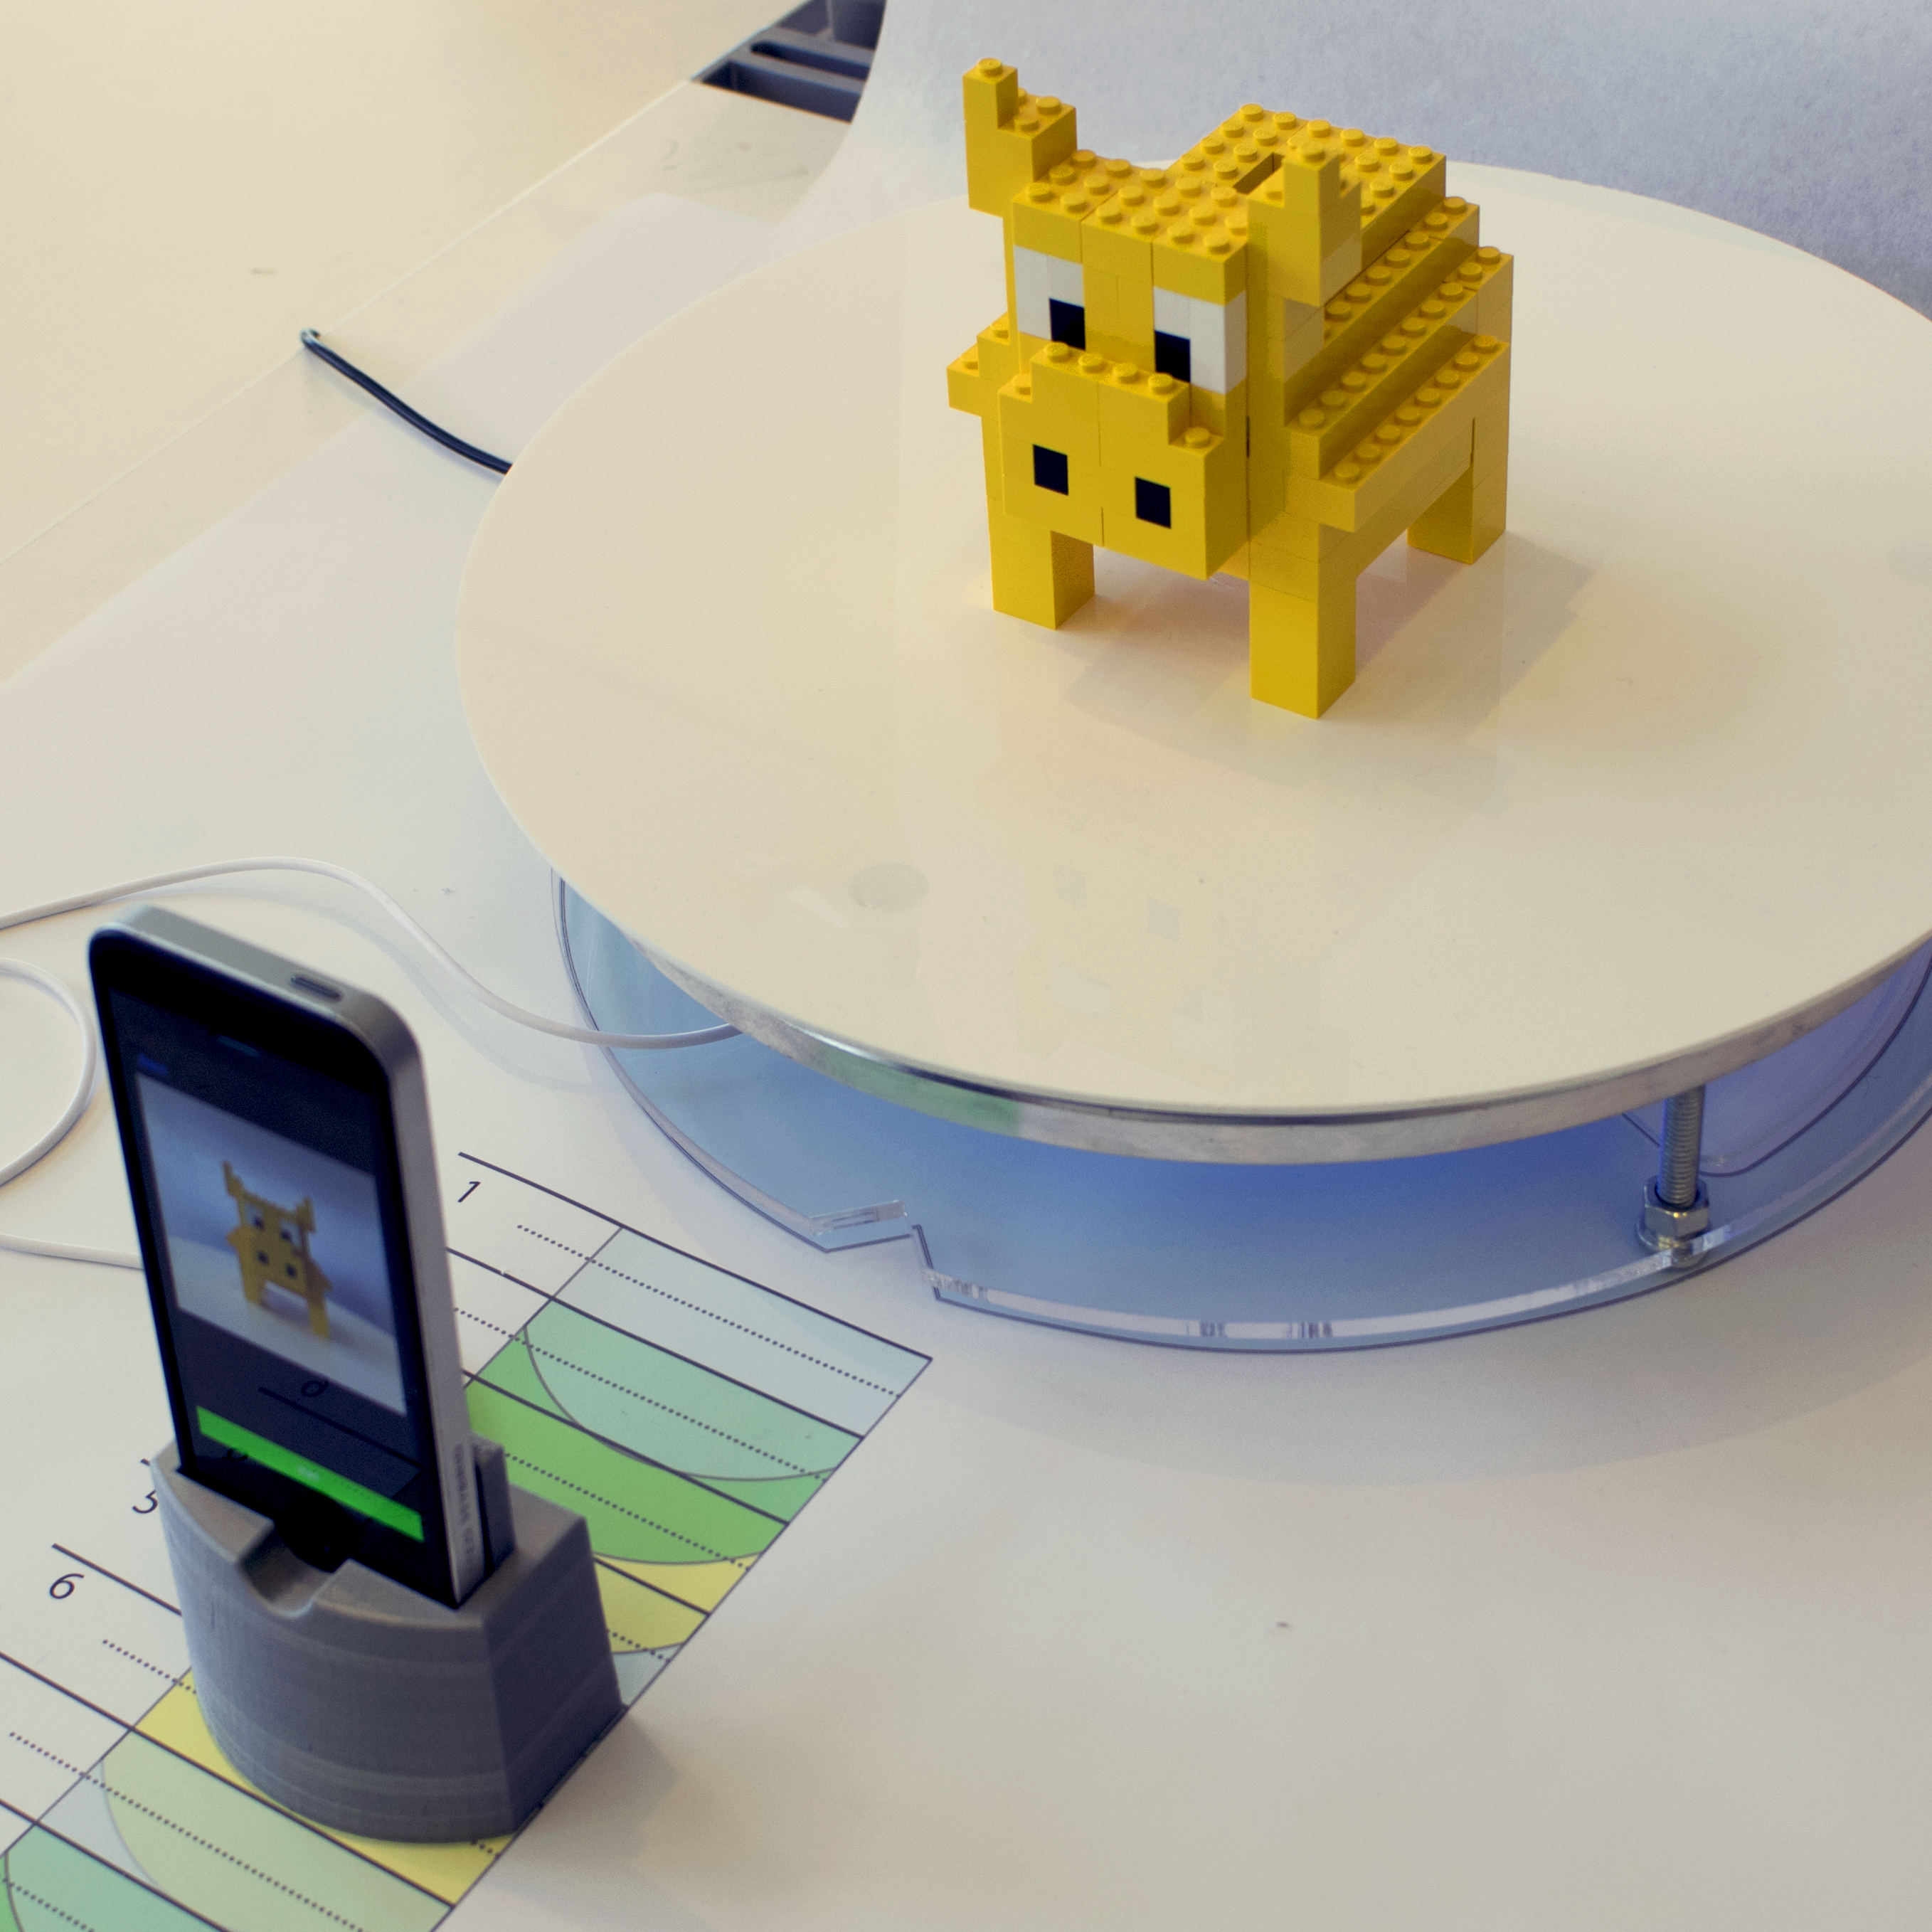
\includegraphics[width=\textwidth]{chap1/spin}               
% 	 \caption{Check it out, it's a Spin margin figure \url{spin.media.mit.edu}}
%  	\label{fig:spin_margin}
%\end{marginfigure}

%\begin{figure}[htb]
% 	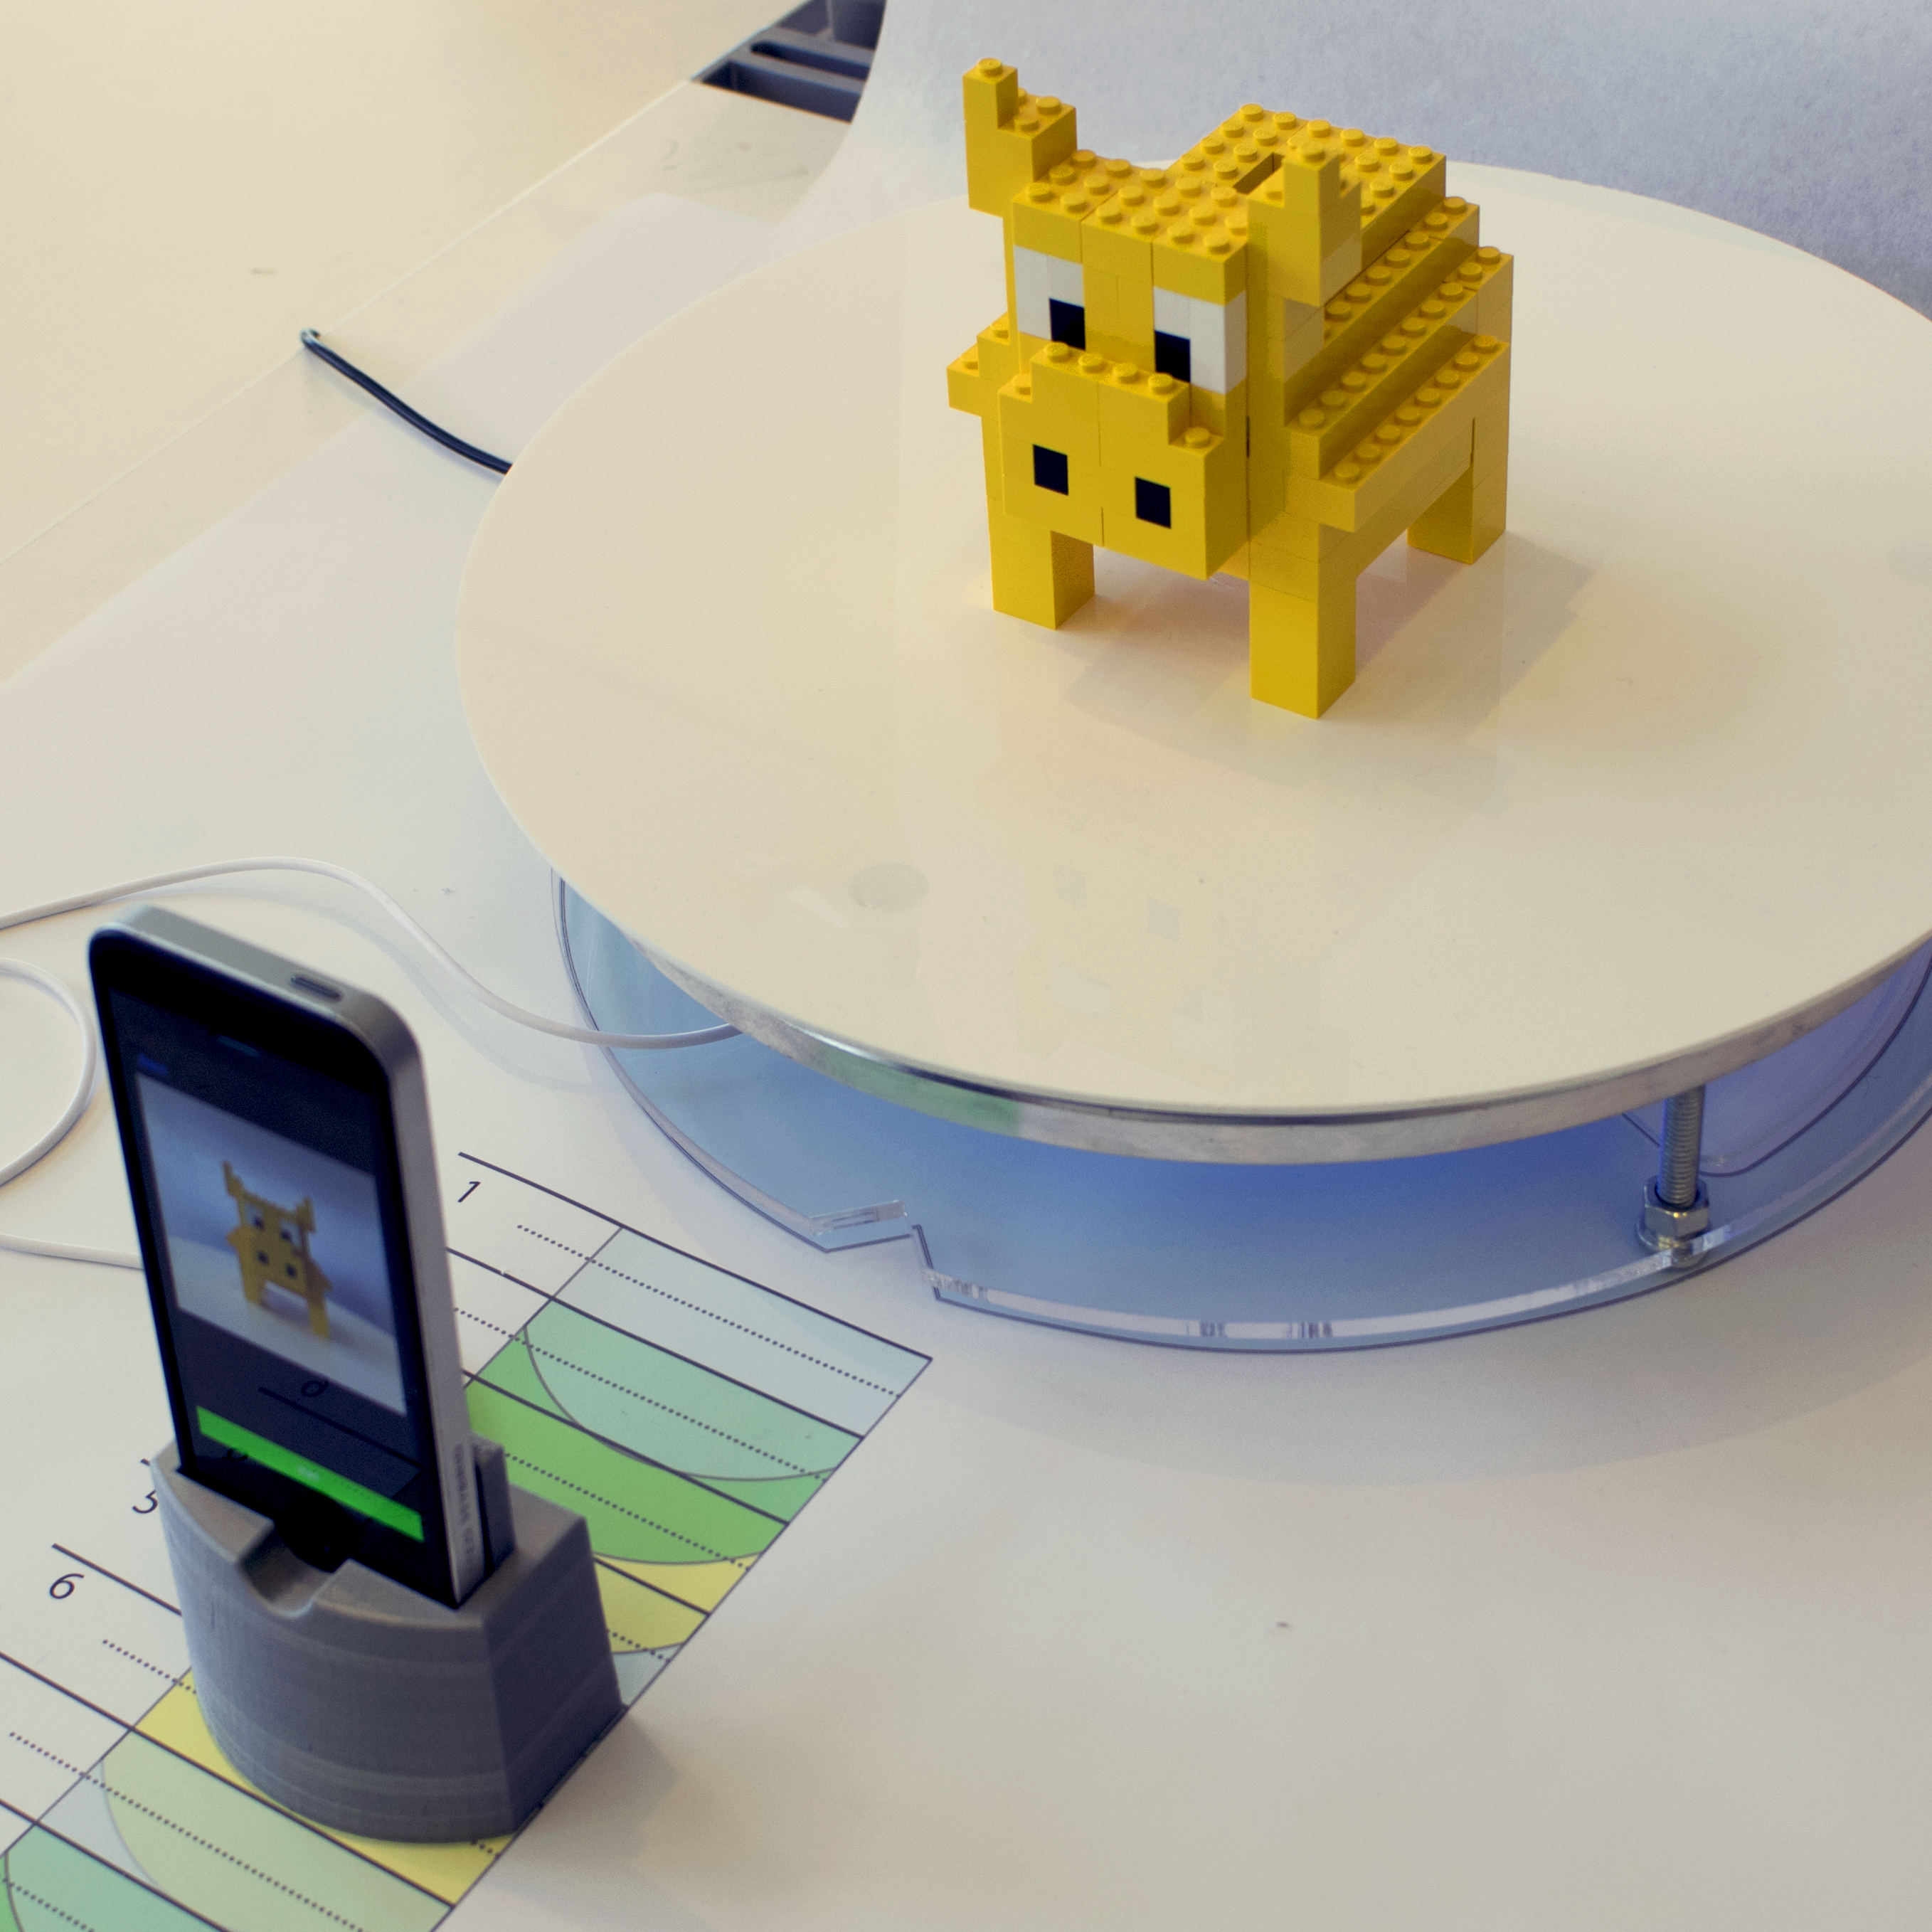
\includegraphics[width=\textwidth]{chap1/spin}               
% 	 \caption{Check it out, it's a Spin \url{spin.media.mit.edu}}
%  	\label{fig:spin}
%\end{figure}
